\documentclass[a4j, 10pt, twocolumn]{ltjarticle}  % 「ltjsarticle」は見た目変わるので注意
\usepackage{amsmath, amssymb, amsfonts}
\usepackage{bm}
\usepackage{color}
\usepackage{cuted}
\usepackage{float}
\usepackage{graphicx}
\usepackage{wrapfig}
\usepackage{luatexja}
\usepackage{luatexja-fontspec}
\usepackage{luatexja-otf}
\usepackage{latexsym}
\usepackage{lltjext}
\usepackage{xcolor}
\usepackage{needspace}
% \usepackage{nidanfloat} 
\usepackage[normalem]{ulem}
\usepackage{tabularx}
\usepackage[hyphens]{url}
\usepackage{here}
\usepackage{multirow}

% ==============================================
% ページ設定のレイアウト確認
% \usepackage{layout}
% 本文中で「\layout」を呼び出す
% ==============================================
% ページ設定
% documentclass「a4j (210*297mm)」を基準とする
% 1inch = 72pt = 25.2mm
% 1pt = 0.35mm
\columnsep=10mm  % 2段組の中央の間隔
\oddsidemargin=-5mm  % 左部の余白領域を小さくする(2段組の5mm)
\evensidemargin=-5mm  % 右部の余白領域を小さくする(2段組の5mm)
\textwidth=17cm  % 本文領域の広さ
\marginparwidth=0mm  % Margin Notesの領域
% ==============================================
% 本文 
\begin{document}
    
    % \layout
    \onecolumn
    \renewcommand{\thepage}{\roman{page}}
    \setcounter{page}{1}

     % 梗概 (Ja)
\section*{梗概}
    \par fugafuga
  % 梗概 (Ja)
    % 梗概 (En)
\section*{Abstract}
    \par hogehoge
  % 梗概 (En)
    \clearpage
    % 謝辞
\section*{謝辞}
    \label{謝辞}
    \par
  % 謝辞
    \clearpage

    % debug
    全体進捗:\textcolor{orange}{12\%}
    
    \tableofcontents  % 目次
    \clearpage
    \newpage

    \twocolumn
    \renewcommand{\thepage}{\arabic{page}}
    \setcounter{page}{1}
    \pagestyle{headings}

    % 第1章
\section{はじめに}
  \label{sec:はじめに}
    \par 近年,欧米や中国を中心に,世界的にシェアサイクルサービスが急速に普及しており,持続可能な交通手段として大きな注目を集めている.これらのサービスは,利用者が好きなタイミングで好きな期間,自転車を利用できるという利便性を提供しており,都市部における交通渋滞の緩和や環境負荷の軽減に寄与している.実際に,世界の主要都市ではシェアサイクルの導入により,大気汚染の削減や健康増進効果も報告されており,その社会的・経済的な効果は無視できないものとなっている.
    \par しかし,既存のシェアサイクルサービスは主に企業が運営するBtoC(Business to Consumer)型モデルであり,その運用にはいくつかの課題が存在している.例えば,都市部と比較して人口の少ない地方では,駅前などの比較的栄えている一部の地域でのみサービスが展開されている場合が多く,地方全体としてはまだまだ普及していないという現状がある.その原因として,事業者がステーションやポートを設置する必要があり,その初期投資や維持管理コストが高額になるため,利用者数の少ない地域では採算が取れず,サービス展開が困難であることが挙げられる.結果として,需要の高い場所にステーションが集中し,郊外やニッチな需要に対応できていない状況が生まれている.
     \par また,都市部においても,シェアサイクルの利用は特定の時間帯や場所に偏りがちであり,それに伴い自転車の不均衡な分布が発生している.具体的には,通勤・通学時間帯には駅周辺の自転車が不足し,逆にオフィス街や学校周辺では自転車が過剰になるといった現象が見られる.これにより,必要な場所に自転車がない,あるいは不要な場所に自転車が集中するといった問題が生じている.事業者はこの不均衡を解消するために,自転車の再配置(リバランス)を行う必要があり,これには追加のコストと労力がかかる.このコスト増加は,サービス料金に反映される可能性があり,利用者の負担増加やサービス品質の低下につながる懸念がある.
      \par 一方,地方部においてもシェアサイクルサービスを利用したいという需要は確実に存在していると考えられる.例えば,公共交通機関が不足している地域では,最寄りのバス停や駅までのアクセス手段として自転車のニーズが高い.また,高齢化が進む地域では,高齢者の移動手段として電動アシスト自転車の需要が増えており,これらのニーズに対応できるシェアサイクルサービスの提供が望まれている.
       \par このようなBtoC型シェアサイクルの課題を解決するために,個人が所有する遊休自転車を有効活用するCtoC(Consumer to Consumer)型シェアリングエコノミーが注目されている.CtoC型シェアリングエコノミーは,消費者同士が直接的に資産を共有することを特徴とし,遊休資産の活用や柔軟なサービス提供,初期投資や運営コストの削減といったメリットが期待される.特に,シェアサイクルの分野においても,CtoC型モデルを導入することで既存のBtoC型モデルが抱える課題を解決できる可能性がある.
       \par 具体的には,自転車を借りる立場からのシェアサイクルだけでなく,自転車を貸す立場からのシェアサイクルにも一定数の需要があると考えられる.例えば,自転車を所有しているが,普段ほとんど使用することがなく,駐輪場や自宅で眠っている自転車を有効活用したいと考える人々がいる.これらの遊休自転車をシェアサイクルサービスの一部として他人に貸し出すことで,所有者は副収入を得ることができ,利用者は必要なときに手軽に自転車を借りることができる.このような相互に利のある関係を構築することで,自転車の有効活用が促進される.
       \par さらに,使われていない自転車が増加することによる駐輪場の不足や放置自転車の問題の解決にもつながる可能性がある.環境面でも,資源の有効活用や廃棄物の削減といった効果が期待できる.加えて,個人所有の自転車は都市部と地方の双方に存在しており,その分布は比較的均一であるため,地域の偏りなくサービスを展開できる可能性が高い.
        \par あらゆる地域に散在している個人所有の自転車をモビリティのリソースとして有効活用できれば,交通手段の多様化と効率化が促進され,地方における交通弱者の支援や,観光地での移動手段の提供など,多面的な効果が期待できる.また,都市交通の混雑緩和や環境負荷の軽減にも寄与し,持続可能な社会の実現に貢献できるのではないだろうか.
        \par しかし,CtoC型シェアサイクルを実現するためには,いくつかの課題も存在する.例えば,貸し手と借り手の間での信用問題や,自転車のメンテナンス・安全性の確保,事故発生時の保険対応などが挙げられる.これらの課題を克服するためには,適切なプラットフォームの構築や法律・規制の整備,そしてユーザー教育が必要である.
        \par そこで本研究では,、このCtoC型シェアサイクルに着目し,その可能性を探求し,その導入に向けた課題と解決策を検討する.具体的には,既存のシェアサイクルサービスの分析からユーザー調査,プラットフォームの設計・開発,および実際のデータを用いたシミュレーション実験を通じて,CtoC型モデルの有効性と実現に向けたきっかけとなることを目的とする.この研究により,持続可能な交通手段としてのシェアサイクルサービスの更なる発展に寄与し,地域社会の活性化や環境問題の解決に貢献したいと考える.
        \par 前述したように,地方でシェアサイクルサービスが普及しない原因として採算性が悪い点が考えられる.しかし,個人所有の自転車をシェアする場合については,予めシェアするための自転車を用意する必要が無いため,初期費用がかなり抑えられることが期待される.また,個人所有の自転車を駐輪している駐輪場が,一般的なシェアサイクルサービスにおけるポートのような存在になるため,新しくポートを確保するための手間や費用も抑えられる.なおかつ,あらゆる場所をポートととして捉えることができる.
        \par 加えて,個人所有の自転車をシェアするサービスを利用することで,自転車を貸す側にもインセンティブが入る.これは,自転車のオーナーが自転車を利用していない時間にお金が入ることを意味する.つまり,シェアサイクルサービス全体の初期費用が抑えられる上,自転車を借りる側にも貸す側にもメリットがあることとなる.価格設定に関しても自転車のオーナーとサービスのユーザー間での調整によって決定することも可能となるため,従来のシェアサイクルサービスに比べて,利用料金の自由度が高いことも特徴的な面になる.
        \par 研究アプローチとしては,まず,システムの利用者のニーズやシナリオ等を定義するユーザー要件や,システムの機能面における必要動作を定義する機能要件,システムの機能以外の面におけるシステムの振る舞いを定義する非機能要件に大別し,それぞれを明確に定義し,サービスにおけるビジネスやシステムの全体像の設計を行う.次に,自転車に取り付けるためのスマートロックのプロトタイプを開発する.ESP32マイコンやサーボモータ,NFCタグや指紋認証センサなどのハードウェアモジュールを用いて実装する.NFCと指紋認証に2つの認証方式を実装し,それぞれで解錠・施錠処理の実現を目指している.続いて,自転車の効率的な割り当てを実現するための整数線形計画法による数理最適化モデルを定式化し,数理最適化ベースの自転車割り当てモデルを構築する.ここでは,SCIPソルバーを用いてモデルを実装し,最適解を求める処理を担う.実際のニューヨーク市内のタクシートリップデータを用いたシミュレーション実験を行い,提案も出るの有効性を検証する.数理最適化ベースの割り当てモデルの他,ランダム割り当てモデルや最近傍割り当てモデル,逐次最適化割り当てモデルなどの複数の比較対象モデルも同時に構築し,提案モデルとの性能比較も行っている.構築した割り当てモデルを利用するためのインターフェースとしてAPIの開発とデプロイも実施している.PythonのFastAPIフレームワークを用いてREST APIを構築し,APIドキュメントの作成とテストを行うことで,APIの品質と信頼性を向上させることに努めた.また,Dockerを用いてAPIをコンテナ化し,クラウド環境にデプロイしている.
        \par 最後に,本論文の構成を説明する.本論文ではまず,\ref{sec:関連研究}章にて本研究の関連研究をまとめる.シェアサイクルやシェアリングエコノミー,スマートロックやマッチングアルゴリズム,API設計に関する既存の研究等をレビューし,本研究の立ち位置を明確にする.特に,BtoC型シェアサイクルの課題とCtoC型シェアリングエコノミーの動向の分析に注力している.\ref{sec:CtoCシェアサイクルのサービス設計とビジネスモデル}章では,本研究で提案するCtoC型シェアサイクルサービスの全体像やコンセプト,サービス設計やコア技術の活用,ビジネスモデルについて詳述する.ユーザーエクスペリエンス(UX)を考慮したペルソナ設計やユーザーシナリオについても説明する.\ref{sec:システム設計}章では,システム要件の定義や全体のアーキテクチャにはじまり,データフローやスマートロックの設計,数理最適化マッチングモデルやAPIの設計について説明する.この章にて機能要件や非機能要件についても定義する.\ref{sec:実装}章では,スマートロックプロトタイプから数理最適化モデルやAPIの実装まで,具体的な手順やコード例を説明する.利用したプログラミング言語やライブラリ,フレームワークについても言及する.\ref{sec:評価と結果}章では,数理最適化モデルの評価やシミュレーション結果,テストケースによる検証を行い,その結果をまとめる.\ref{sec:考察}章では,主に\ref{sec:評価と結果}章の結果を参照し,システム全体の有効性やCtoC化によるメリット・デメリットなど,その結果から得られる考察をまとめる.

  % 第1章
    \clearpage
    \newpage
    % 第2章
\section{関連研究(\textcolor{green}{100\%})}
  \label{sec:関連研究}
    \par
  
  \subsection{シェアサイクルの現状と課題(\textcolor{green}{100\%})}
    \label{sec:シェアサイクルの現状と課題}
      \par シェアサイクルは,都市部を中心に世界各地で普及している持続可能な交通手段であり,そのビジネスモデルは主にBtoC型である.本節では,これらのモデルの現状と課題について検討し,特にBtoC型シェアサイクルの限界とCtoC型シェアリングエコノミーの動向に焦点を当てる.
      \par シェアサイクルの分野でも,CtoC型モデルを導入することによって,BtoC型のシェアサイクルビジネスモデルが抱える課題を解決し得る可能性がある.遊休自演者の有効活用や,需要に応じた柔軟なサービス提供,初期投資や運営コストの削減など,CtoC型ならではのメリットが期待される.
      
      \subsubsection{BtoC型シェアサイクルの限界(\textcolor{green}{100\%})}
        \label{sec:BtoC型シェアサイクルの限界}
          \par BtoC型(Business-to-Consumer)シェアサイクルとは,事業者が自転車を保有および運営し,利用者がそのサービスを利用して自転車を借りるというビジネスモデルである.BtoC型では,特定の企業や自治体が自転車を大規模に保有・管理し,ユーザが自転車が駐輪されているステーションや無人ポートから自転車を借りる.欧米やアジアなどの大都市を中心として世界的に普及しており,代表的なサービスに,日本のドコモ・バイクシェア,アメリカのCiti Bike,イギリスのSantander Cycles,フランスのVelib’などが挙げられる.
          \par しかし,BtoC型シェアサイクルにはBtoC型であるが故の課題を抱えている.特に初期投資や運営に係るコストの高さや,地理的・時間的再配置の難しさ,自転車ポートの配置や柔軟性・拡張性の制約などが挙げられる.
          \par 世界の40都市における自転車シェアリングシステムの空間的な分布,公共交通機関との統合,および全体的な有効性を分析したMahajan氏らの研究\scalebox{0.7}{\cite{bike-sharing-accessibility}}では,自転車シェアリングサービスのアクセシビリティを評価するための新しい指標であるBSAI(Bike-Share Service Accessibility Index)を導入し,シェアサイクルサービスの利用のしやすさやパフォーマンスを定量的に評価した.
          \par BSAIが高い都市の例として,トロントやワシントン,チューリッヒなどが挙げられている.これらの都市は,広範なサービス範囲や公共交通機関との統合,効率的なインフラ投資を行っているという特徴を持っている.一方で,BSAIが低い都市のの例として,オースティンやサンアントニオなどが挙げられている.これらの都市は,サービス範囲が限定している点や,公共交通機関との連携不足,非効率的なインフラ投資などの課題を持つ点に共通している.
          \par この研究が示唆している課題は,自転車シェアリングシステムのインフラが,都市のすべての住民に公平にアクセス可能ではない点にある.自転車ステーションやポートの分布には地域格差があり,特にBSAIが低い都市ではポートの設置範囲や数が限定されている.それにより,自転車ステーションやポートが特定のエリア内においてのみ利用可能であるため,ユーザのアクセシビリティが悪化している.また,公共交通機関との連携が不足している点も,サービス範囲が限定している点に起因すると考えられる.ただ,BtoC型シェアサイクルでは,企業は利益のために,需要の高い地域に自転車ステーションやポートを設置するはずであるため,必然的な課題とも捉えられる.設置エリア外への展開が難しく,郊外やニッチな需要には対応できない点もBtoC型シェアサイクルの課題である.
          \par また,自転車シェアリング事業の長期的な成功のための政策とビジネス上の教訓を提示することを目的としNikitas氏の研究\scalebox{0.7}{\cite{nikitas2019save}}では,スウェーデンとギリシャでのアンケート調査と,世界各地の自転車シェアリングの成功例と失敗例の分析を組み合わせ,その知見を導き出している.
          \par この研究では,既存の自転車シェアリング事業の成功と失敗の事例を詳細に分析し,その要因を特定している.例えば,アメリカで初めてドックレスバイクシェアシステムを提供した中国のバイクシェアリング企業Bluegogo社は,過剰な自転車供給と需要不足のため,2017年11月に経営破綻した.北京大学発のスタートアップOfo社も,英国事業が赤字となり,2019年1月には3,000台を保有していたロンドンから撤退することとなった.
          \par これらは論文で紹介されいてる事例の一部にすぎないが,この研究が示唆している課題に,過剰共有が挙げられる.ドックレスバイクシェアリングの急速な拡大に伴い,多くの都市で自転車が過剰供給されており,需要と供給のミスマッチが生じていると考えられる.しかし,BtoC型シェアサイクルにおいては,サービスを提供するために大規模な自転車を事前に用意する必要があるため,避けがたい課題である.
          \par さらに,地理的・時間的な再配置の難しさについても言及されている.ドックレスバイクシェアリングの導入によって,従来のステーションベースでは不可能であった乗り捨てによるドアツードアの利便性が向上した.その一方で,ユーザによって利用時間帯や場所が偏るため,自転車の分布が不均一になりやすく,需要のある場祖に自転車が不足する,または需要のない場所に自転車が過剰に集中するという課題が発生している.自転車が供給されないまま放置されていると,ユーザのアクセシビリティ低下を招くほか,景観を損ねるなどの,ユーザ以外への影響も懸念される.そのため,定期的に自転車の再配置を行う必要がある.しかし,再配置には人力・トラック等が必要であり,コスト増加やオペレーションの難化を招いている.

      \subsubsection{CtoC型シェアリングエコノミーの動向(\textcolor{green}{100\%})}
        \label{sec:CtoC型シェアリングエコノミーの動向}
          \par シェアサイクルのBtoC型モデルにて例示した課題を受け,様々な事業ドメインにおいてCtoC型シェアリングエコノミーが注目されている.本研究の研究領域であるCtoCシェアサイクルもCtoC型シェアリングエコノミーの一部として捉えることができるため,本項でCtoC型の特徴や動向をまとめ,俯瞰することとする.
          \par まず,CtoC型シェアリングエコノミーを定義するにあたり,Frenken氏らの研究\scalebox{0.7}{\cite{frenken2019putting}} が参考になる.この研究では,シェアリングエコノミーの定義を明確にし,その経済的,社会的,環境的影響を評価し,既存の規制と代替プラットフォームの構造について考察している.Frenken氏らは,シェアリングエコノミーを「消費者が,一時的に,余剰の物理的資産(遊休能力)を,場合によっては金銭を介して相互に利用し合うこと」と定義している.
          \par この定義は,従来の共有の概念とは異なり,特に消費者間の取引であることや遊休能力の活用などが強調されている.つまり,ここで定義しているシェアリングエコノミーは,企業を介さず,消費者同士が直接的に資産を共有し,その共有する資産は,所有者が常に使用しているわけではない余剰の資産(例えば,空いている部屋や使っていない自動車)が共有されることを意味している.ただし,企業はプラットフォーマーとして間接的に取引に介在する可能性はある.これはインターネットプラットフォームの登場により,「見知らぬ者同士の共有(stranger sharing)」という概念が生まれたためである.
          \par シェアリングエコノミーの性質,運営メカニズム,および伝統的な経済理論と市場運営への影響を経済学の観点から詳細に分析することを目的としたChen氏の研究\scalebox{0.7}{\cite{AnalysesAndPerspectivesFromAnEconomicPerspective}}では,具体的な事例分析を通してシェアリングエコノミーの実態を明らかにしている.CtoC型シェアリングエコノミーのプラットフォーム型ビジネスの例として,UberとAirbnbが挙げられる.Uberは,都市交通の分やでドライバーと乗客を結び付け,交通手段の効率化と柔軟な移動オプションを提供し,Airbnbは,住宅所有者が空き部屋を旅行者に貸し出すことを可能にし,宿泊業界に新たな選択肢をもたらした.このような事例から,CtoC型のシェアリングエコノミーおよびそのプラットフォームは,遊休資産を有効活用することで新たな価値を創出し,消費者の行動や産業構造を変化させ,今日の隆盛を迎えるまで成長を遂げてきた.
          \par このCtoC型シェアリングエコノミーの成長と促進の要因は,技術や社会,経済など多岐にわたる.
          \par 協調消費(Collaborative Consumption)への参加を促す動機を調査し,持続可能性や楽しさ,評判や経済的利益といった要因が,協調消費に対する態度や行動意図にどのように影響するかを分析したHamari氏らの研究\scalebox{0.7}{\cite{hamari2016sharing}}では,技術や社会,経済のそれぞれの観点からその要因について言及されている.
          \par 情報通信技術の観点においては,Web2.0の発展により,ユーザ生成コンテンツの増加やオンラインでの共同作業が容易になった点やオンラインプラットフォームを通じて物品やサービスの共有が促進された点,またそれらによってオープンソースソフトウェアやP2Pファイル共有などの様々な形態のシェアリングエコノミーが生まれたことがシェアリングエコノミーの成長要因として挙げられる.
          \par 経済的観点においては,所有することよりもアクセスできることを重視し,必要な時に必要な分だけ利用することに対する消費者の価値観の変化がシェアリングエコノミーの成長を後押ししている.また,CtoCプラットフォームは,従来のサービスよりも安価にサービスを提供できることが多く,消費者にとって魅力的な選択肢となる.例えば,Airbnbはほてるよりも安価な宿泊施設を提供し,Uberはタクシーよりも手頃な価格で移動手段を提供できる場合がある.また,これはユーザだけでなく,提供者としての個人が自分の遊休資産を貸し出すことによって収入を得る機会を提供することにもなる.これによって個人が新たな収入源を確保し,経済的な自立を促進できることも成長要因として挙げられる\scalebox{0.7}{\cite{sundararajan2017sharing}}.
          \par 社会的観点においては,オンラインプラットフォームにおけるユーザレビューや評価システムが,見知らぬ人同士の取引における信頼を構築する上で重要な役割を果たし,個人間でもスムーズに取引が可能となった点が成長要因として挙げられる.また,環境問題意識への関心の高まりから,環境負荷を低減するために持続可能な消費を求める消費者が増加している点も起因していると考えられる.
          \par 本研究とは異なる事業ドメインで構築されているシェアリングエコノミーから着想を得ることで,シェアサイクルの事業ドメインでも応用可能性があると考えられる.
      
  \subsection{スマートロック技術の進展(\textcolor{green}{100\%})}
    \label{sec:スマートロック技術の進展}
      \par 近年,IoTデバイスの普及に伴い,スマートロック技術は急速に発展してしている.特に,スマートロック技術は,シェアサイクルサービスの実現において重要な役割を果たし,ユーザエクスペリエンスの向上や運用効率の最適化に不可欠な要素となっている.本節では,その技術的進展について,ハードウェアの最新動向およびセキュリティと信頼性の二つの観点から検討する.

      \subsubsection{ハードウェアの最新技術(\textcolor{green}{100\%})}
        \label{sec:ハードウェアの最新技術}
          \par 前節で言及したBtoCやCtoCモデルへの課題や特徴を踏まえ,本項では,それらを実現・強化するうえで必要となり得るハードウェア技術がどのように発展し,今日を迎えているのかについて理解するため,特にCtoCシェアサイクルサービスに関連するハードウェア基盤の最新動向を概観する.
          \par IoTデバイスのエッジで機械学習(ML)モデルを実行するためのTinyML as a Service(TMLaaS)アーキテクチャを提案したZaidi氏らの研究\scalebox{0.7}{\cite{zaidi2022unlocking}}では,小型で低消費電力MCU(Micro Controller Unit)の発展について触れられている.実際に市販のIoT MCUの消費電力と利用可能なメモリを比較し,理想的にはローカル計算機能を提供するため,RAMやFLASHなどのオンボードメモリが多く,消費電力の低いMCUが必要とされるものの,これらの要件を同時に満たす商用製品は存在しないとまとめられている.しかしそれでも,最近のESPやSTM,NINA,Nano BLE Senseなどのシリーズは,より高性能でありながら低消費電力を実現しており,設計するにあたってよりよい選択肢となる.
          \par また,組み込みAIやエッジコンピューティングの分野では,AI推論用アクセラレータや小規模ニューラルネット処理が可能なMCUの登場によって,デバイス上での状態判定が実現可能になっている.これはMCUの進化のほか,リソース制約のあるデバイスでMLモデルを開発・実行するためのツールを提供するTinyMLフレームワークや,MCU上でMLを実行するための統一フレームワークであるTensorFlow Lite Micro,ニューラルネットワークモデルの計算量とストレージ要件を削減するための様々なモデル圧縮技術の発展によって実現可能となった.具体的な応用例として,製造業では,振動パターン分析による機械の故障の事前検知やセンサ推論に基づくデバイス制御の自動化,スマート農業では,環境データに基づく農業技術の最適化や,植物の病気の早期検出などが挙げられる.これはシェアサイクル業界においても,振動センサから取得したデータに基づく自転車の状態監視や,加速度センサを用いた自転車の不審な動き検知および盗難の防止にも応用が可能であると推察される.
          \par LPWAN(低電力広域ネットワーク)LoRa/LoRaWANシステムの可能性に焦点を当てているMilarokostas氏らによる研究\scalebox{0.7}{\cite{milarokostas2022comprehensive}}では,LPWAN技術,特にLoRa/LoRaWANシステムに関する包括的な調査を提供しており,通信技術に関する動向を知ることができる.LPWANとは,IoTエコシステムをサポートする主要な候補であり,エネルギー効率が高く,費用対効果の高い技術を組み込んでいるため,IoTサービスプロビジョニングに適している.免許不要のスペクトラム上で無線アクセスを提供する有力なソリューションであるLoRa/LoRaWANや,3GPP(3rd Generation Partnership Project)によって策定されたセルラーIoT(CIoT)技術であり,ライセンススペクトラムを使用するNB-IoTなどがLPWAN技術の例として挙げられる.
          \par これらのLPWAN技術によって,エンドデバイスへのコマンド送信を可能とし,遠隔からのロック制御などの操作も可能となる.さらに,LoRaWANシステムにおいては,ネットワークサーバが位置情報サーバなどの追加コンポーネントを提供できると言及されていることから,位置情報サービスもLoRaWANの応用事例の1つであることが示唆される.これらの技術は,シェアサイクル事業において必要となるGPS追跡や遠隔ロック制御を容易にする基盤技術を提供していると言える.
          \par 通信モジュールやセンサーボード,電源ユニットが標準化され,用途に応じて組み合わせるプラットフォーム的アプローチが容易になっている点もハードウェア技術の進歩に寄与していると考えられる.オープンソースハードウェア(OSH)におけるモジュール性の概念を,デザイン,製造,ハードウェア,コミュニティなど,さまざまな側面から分類し,それぞれのモジュール性を定量的に評価したGavras氏らによる研究\scalebox{0.7}{\cite{Gavras_Kostakis_2021}}では,従来の製品設計の文献で議論されてきたモジュール性とは異なるOSH特有の,無形デザインモジュール性や製造モジュール性などのを提示し,これらのモジュール性がOSHの開発において重要な役割を果たしていることを明らかにしている.
          \par また,ArduinoやRaspberry Pi,ESP32などの開発者コミュニティが拡大し,試作から実用までの開発プロセスが短縮されている点や,第三者が作成した多くのOSHプロジェクトを閲覧できるプラットフォームが発達してきた点も,今日のハードウェア技術基盤を構築する要素になっているに違いない.
      
      \subsubsection{セキュリティと信頼性の確保(\textcolor{green}{100\%})}
        \label{sec:セキュリティと信頼性の確保}
          \par スマートロックを含むIoTデバイスにおいてセキュリティリスクや信頼性確保の観点は非常に重要である.特に,本研究の事業ドメインであるシェアサイクルにおいて,機密性や完全性,可用性を以下に守るのか,CtoCサービスでユーザ間の信頼をどう醸成するのかという視点から関連する研究をまとめる.
          \par スマートロックのセキュリティについて調査し,特にMaster LockのBluetoothパッドロックにおける複数の脆弱性を発見したKnight氏らの研究\scalebox{0.7}{\cite{8887393}}では,APIのセキュリティ問題やゲストアクセス権限の不備など,複数の脆弱性を発見および報告し,IoTデバイスのセキュリティにおけるバックエンドサービスの重要性を指摘している.
          \par Master Lockスマートパッドロックに存在した脆弱性は主にAPIセキュリティ上の脆弱性,一時コードにに関する脆弱性,それ以外の脆弱性の3つカテゴリに分類される.APIセキュリティに関しては,本来オーナのみがアクセスできるはずのプライマリーコードをゲストユーザがAPIを通じて取得できてしまう点や,APIが一度生成されると無期限に有効であり,キーが漏洩した場合にユーザのパスワード漏洩と同等のリスクが存在していた点などに脆弱性が報告された.一時コードに関しては,アプリケーションインターフェース上では一時コードの有効期限が4時間と示されていたものの,実際には8時間有効であるという不一致がある点などが報告された.
          \par これらの脆弱性の中でも,特にAPIの脆弱性が最も深刻であり,アクセス権限が無いはずのユーザでもパッドロックを解錠できるという問題があった.CtoCシェアサイクルスキームにおいても,Master Lockのようなスマートロックを使用するため,この脆弱性に対する策を講じる必要がある.具体的には,オーナやゲストといったユーザのステータスに基づき,厳格なアクセス制御ポリシを実装し,不必要な情報へのアクセスを制限したり,APIの呼び出しに対するレート制限を設け,不正なアクセス思考を防止できるようにしたりするアプローチが有効であるとされる.
          \par IoV(Internet of Vehicles)における信頼性管理と信頼性共有のメカニズムを提案したJing氏らの研究\scalebox{0.7}{\cite{jing2022joint}}では,セキュリティと信頼性の確保のために,複数の側面から取り組んでいる.
          \par 信頼性管理メカニズムに関しては,機械学習技術であるRandom Forestを利用して悪意のある車両を識別し,さらに,経路予測アルゴリズムに基づいた信頼性共有メカニズムを導入することで,ネットワーク全体のセキュリティを強化した.また,スライディングタイムウィンドウ技術を用いて過去と現在の記録に基づき,車両の信頼度を総合的に評価し,一時的な行動だけでなく,長期的な信頼性を考慮した評価を可能とした.
          \par 信頼性共有メカニズムに関しては,集中型のコントローラに依存せず,分散型の信頼性管理アプローチを採用し,単一障害の問題を回避することでシステムの拡張性を高めた.また,信頼性情報はRSU(Roadside Units)間でポイントツーポイントで共有され,中央コントローラの負担を軽減し,ネットワークの拡張性を向上させた.
          \par さらに,この研究では通信のセキュリティにも言及されている.Elliptic Curve Cryptography(ECC),Cryptographic Hadh Function,XOR演算を組み合わせた軽量な暗号化メカニズムを導入し,CMV(Cluster-Member-Vehicles),CHV(Cluster-Head-Vehicles),RSU間の通信を保護している.これによって,リソースの限られたIoTおよびIoV環境でも安全な通信を実現することを可能としている.また,暗号化メカニズムによって通信リンクへの攻撃を防ぎ,データの改ざんや盗聴からも保護する役割を担っている.
          \par これらのセキュリティ対策に関する考え方や技術はCtoCシェアサイクルにおけるセキュリティ対策にも応用可能であると考えられる.
          \par スマートシティの様々なアプリケーションとアーキテクチャを紹介し,それらのセキュリティとプライバシーの課題を議論しているZhang氏らの研究\scalebox{0.7}{\cite{zhang2017security}}では,屋外利用のシェアサイクルにも適用可能なセキュリティ設計に関する知見を得ることができる.特に,スマートシティでは,様々なセンサやデバイスを通じてデータが収集され,その中でも位置情報が不可欠な情報として収集される.実際にサービスを提供する際には利用者の同意を得た上で位置情報を取得することが原則であり,その際にデータ収集の目的を明確化し,必要最小限のデータのみを収集するように設計することが求められる.
          
  
  \subsection{マッチングアルゴリズムの研究動向(\textcolor{green}{100\%})}
    \label{sec:マッチングアルゴリズムの研究動向}
      \par 本節では,シェアサイクルにおける需要と供給を効率的に結びつけるためのマッチングアルゴリズムの研究動向について整理する.マッチングアルゴリズムは,利用者と自転車,自転車と駐輪場,さらにはリソースの最適な割り当てなど,シェアサイクルの運用効率やサービス品質を向上させる上で重要な役割を果たしている.
      \par マッチング問題は,多岐にわたる分野で研究されており,具体的なアプローチとして数理最適化手法と機械学習手法が挙げられる.数理最適化手法では,問題を数奇モデルとして定式化し,制約条件下で目的関数を最適化することで解を求める.一方で機械学習手法では,大量のデータからパターンや特徴を学習し,予測や分類,最適な意思決定を行う.
      \par 本節では,これらの手法がシェアサイクルのマッチング問題にどのように適用されているか,または応用し得るかについて,具体的な研究事例を交えて詳しく述べる.まず,\ref{sec:数理最適化によるマッチング手法}項にて数理最適化によるマッチング手法を取り上げ,その後,\ref{sec:機械学習によるマッチング手法}項にて機械学習によるマッチング手法を概観する.

      \subsubsection{数理最適化によるマッチング手法(\textcolor{green}{100\%})}
        \label{sec:数理最適化によるマッチング手法}
          \par 本項では,荷物の運搬や配車,リソースの割り当てなどの分野でも盛んに研究されている数理最適化を用いたマッチング手法が,シェアサイクルの需要と供給を効率的に結びつけるためにどのように活用されているか,または活用し得るかを整理する.
          \par まず,マッチング問題の基本定義や典型的な最適化手法やそのモデルについて触れる.整数計画法は,一部または全ての決定変数が整数値のみをとるように制約された線形計画法であり,組み合わせ最適化問題の1つとして広く認知されている\scalebox{0.7}{\cite{wolsey2020integer}}.例えば,荷物の配送計画や工場の生産計画,従業員のシフトスケジューリングなどでは,それぞれ「トラックを何台稼働させるか」「対象製品を何個生産するか」「対象日に従業員を何人割り当てるか」などの問題を解く必要がある.これらは変数が連続値ではなく整数値でなければならない.こうした「整数値でなければならない」という制約を直接扱うための手法が整数計画法である.
          \par 一方で,線形計画法では,決定変数を連続変数として扱うことができるため,ある問題に対して線形計画法によるアプローチで解こうとすると,変数は整数値以外も取ることができる.そのため,本研究でアプローチしているような整数計画問題を線形計画法を用いたプロセスで処理しようとすると,線形計画法による解が整数ではない場合,丸めた解が実行不可能または最適ではない可能性がある\scalebox{0.7}{\cite{hooker2024integer}}.これは,事前に考慮した制約条件の基づき厳密に解を算出した場合でも,丸めてしまうことでとたんに制約条件を満たさない解になる可能性が十分考えられるからである.
          \par このような数理最適化によるマッチング問題を拡張することで,様々な問題にアプローチすることができる.マッチング問題を,選好リストが明示的に与えられる明示的マッチングと,選好リストを予測する暗黙的マッチングの2つに分類し,それぞれの問題に対するモデルとアルゴリズムを包括的にレビューしたRen氏らの研究\scalebox{0.7}{\cite{9416305}}では,特に,検索やユーザとアイテム,エンティティ同士の関係,画像マッチングなどの暗黙的マッチングにおける多様なアルゴリズムを網羅的に扱い,それぞれの応用例と技術的課題について言及されている.
          \par 選好リストが明示的に与えられる明示的マッチングでは,エージェントは合理的かつ利己的であると仮定され,明示的に与えられたランキングとして選好リストを保持している.経済学や数学の分野で主に研究され,結婚市場や医療インターンのマッチングなどが例として挙げられている.安定したマッチングを求める問題に対して用いられることが多い.一方で,選好リストを予測する暗黙的マッチングでは,エージェントの選好は,ユーザーの行動履歴やアイテムの特徴などから推測されるため,データの収集と分析,マッチングスコアを計算するプロセスが重要になる.選好リストを生成するために類似度計算や機械学習が用いられ,ニューラルネットワークなどのアルゴリズムを実装する必要があるマッチング問題で用いられることが多い.より詳細な内容は\ref{sec:機械学習によるマッチング手法}項にて触れるため,適宜参照されたい.
          \par これらの概念は,数理最適化によるマッチング手法をシェアサイクル分野へ応用する際に役立つ可能性がある.明示的マッチングとしては利用者と自転車のマッチングや駐輪場と自転車のマッチングなどのが考えられる.利用者が希望する自転車の条件を考慮した上でマッチング処理を行うことで,より満足度の高いサービスを提供できる.CtoCシェアサイクル領域では特に乗り捨て場所の考慮が重要になるが,これも利用者の目的地と自転車の所有者の位置などを選好リストとして保持することで明示的マッチングが可能となる.
          \par 暗示的マッチングとしては,利用者への自転車の推薦や需要予測と自転車配置の最適化などが挙げられる.利用者の過去の利用履歴や移動パターン,利用時間帯や天気などの様々な情報から,個々の利用者に合った自転車を推薦する際に役立つ.また,シェアサイクルサービス全体としての過去の利用データから需要を予測し,自転車の再配置の最適化などに応用できる可能性も考えられる.
          \par ただ,数理最適化問題を解く際にはNP困難性について考慮しなければならない.NP困難な巡回セールスマン問題を解くため,最短経路や最小全域木などのPクラスのアルゴリズムの知識をニューラルネットワークに組み込むことを試みたGeorgievらの研究\scalebox{0.7}{\cite{np-hard}}では,このNP困難性について触れられている.
          \par 数理最適化におけるNP困難性とは,問題の難しさを示す概念の1つであり,効率的に問題を解くためのアルゴリズムが知られていない問題のことを意味する.問題の規模が大きくなるにつれ,問題を解くための計算量が指数関数的に増加する可能性のある問題である.CtoCシェアサイクルにおける組み合わあせ最適化問題に関しても一般にNP困難問題であることから大規模化するシェアサイクル運用で厳しい計算負荷が生じる可能性がある.そのような場合,従来の数理最適化処理で用いられてきた近似アルゴリズムやヒューリスティックな手法を用い,必ずしも最適ではないかもしれないが,実用的な時間内で十分に良い解を求めるアプローチも選択肢として持っておくべきである.それに加えて,この研究で提案されたニューラルネットワークを用いてNP困難な問題にアプローチする選択肢も存在することを考慮しておけると最適なアプローチを都度選定することができる.
          
      \subsubsection{機械学習によるマッチング手法(\textcolor{green}{100\%})}
        \label{sec:機械学習によるマッチング手法}
          \par 本項では,\ref{sec:数理最適化によるマッチング手法}項にて扱った数理最適化手法と比較し,機械学習を活用したマッチング手法について概観する.
          \par 数理最適化は,モデルに対して制約や目的関数を定義することで処理を行っているのに対し,機械学習では,大量の履歴データやその特徴量からモデルを学習しマッチングなどの処理を行っている.
          \par このようなデータ駆動型アプローチの特徴については,機械学習の観点から最適化手法を体系的に回顧・要約し,最適化と機械学習の研究の両方の発展に指針を与えることを目指したSun氏らの研究\scalebox{0.7}{\cite{8903465}}にて詳しく解説されている.この研究では,多くの機械学習アルゴリズムの本質は,最適化モデルを構築し,与えられたデータから目的関数のパラメータを学習することであると述べられている.ただ,それ故に,データ量が指数関数的に増加し,モデルの複雑さが増すにつれ,機械学習における最適化手法はますます多くの課題に直面するとも指摘されている.
          \par また,データ駆動型アプローチとしての代表的な機械学習の手法についても紹介されている.半教師あり学習は,教師あり学習と教師なし学習の中間の方法であり,学習プロセス中にラベル付きデータとラベルなしデータの両方を組み込む.ラベル付きデータが少ない状況でもラベルなしデータを活用して学習効果を高めることが可能となる.強化学習では,エージェントが試行錯誤メカニズムを通じて環境と相互作用し,累積報酬を最大化することによって最適な戦略を学習する.環境からのデータを報酬として扱い,その報酬に基づいてエージェントが最適な行動戦略を学習する.メタ学習では,少数のサンプルで新しい環境に効率的に適応できるモデルを設計することを目指している.複数のタスクからのデータに基づいて学習モデルを学習する.その他にも,確率的勾配法やその適応型バリアントが使用された深層学習や,観測データに基づいてモデルのパラメータを最適化し,真の事後分布を近似する変分推論なども紹介されている.
          \par これらの機械学習手法を用い,マッチング手法として具体的にアプローチされている例として,ビジネスインテリジェンスにおける機械学習の応用について焦点を当て,それぞれの特性やツールおよび使用原則を定義したNaneva氏らの研究\scalebox{0.7}{\cite{business-intelligence}}にて紹介されている.
          \par 例えば,ソーシャルメディアにおける顔認識が紹介されている.ソーシャルメディアの最適化を目的として,顔認識機能に機械学習が利用されている.写真の中のポーズや投影をスキャンすることでソフトウェア側が適切な提案を行っている.また,交通渋滞の分析に基づき,交通予測を行うために機械学習が利用されている例も紹介されている.機械学習は項宇宙量の多いエリアと少ないエリアを特定し,ユーザの移動を改善するための定期的な予測を作成することができる.
          \par さらに,Poer BIのようなBIソフトウェアでは,自動機械学習が利用されている.これは,レポートに含まれる情報とは別にデータ操作を提供し,最も関連性の高い特徴とアルゴリズムを自動的に抽出し,機械学習モデルの検証を行う.自動機械学習は,二項予測や一般分類,回帰モデルなどの機械学習モデルを適切に選択して,トレーニング,改善,適用という主要な3つのステップを実行することができる.他にもクラウドサービスのAzureを用いたデータ管理と機械学習の活用についての事例なども紹介されている.
          \par これらの例は,機械学習がビジネスインテリジェンスにおいて,最終的な意思決定をどのように支援するのかを示している.本研究の領域であるCtoCシェアサイクル領域においても利用できる可能性が示唆される.実際に機械学習によるマッチング手法をシェアサイクル領域へ応用されている事例も存在する.ワシントンDCの自転車シェアリングの需要予測モデルを改善するため,交通事故の発生件数という新しい特徴量を機械学習の訓練データとして導入し,その有効性を検証したKim氏らの研究\scalebox{0.7}{\cite{PredictionofBikeShareDemandbyMachineLearning}}を紹介する.
          \par この研究では,ランダムフォレスト,XGBoost,LightGBMという3つの機械学習モデルにこの特徴量を加えることで,RMSLEスコアがどうなるかを検証した.なお,RMSLEとは二乗平均平方根誤差を意味しており,予測値と実際の値の誤差を評価するための指標の1つである.具体的な導出式は以下の\ref{equ:RMSLE}式の通りである.なお,\ref{equ:p_i}式と\ref{equ:a_i}式の通り,$p_i$と$a_i$はそれぞれ予測値と実際の値を意味し,$n$はデータ点の数を意味している.

          \begin{equation}\label{equ:RMSLE}
            \sqrt{\frac{1}{n}\sum_{i=1}^n(\log(p_i + 1) - \log(a_i + 1))^2}
          \end{equation}
          
          \begin{equation}\label{equ:p_i}
            p_i = PredictedValue
          \end{equation}

          \begin{equation}\label{equ:a_i}
            a_i = ActualValue
          \end{equation}

          \par 結果として,すべてのモデルにおいてRMSLEスコアが改善したことが示されている.つまり,シェサイクル領域において,機械学習を用いて需要予測を行う際に多かれ少なかれ交通事故の発生件数が影響していることを示唆している.このようにシェアシェアサイクル領域のみに絞っても機械学習の利用方法は多岐に渡る.
          
  \subsection{API設計と都市への適用性(\textcolor{green}{100\%})}
    \label{sec:API設計と都市への適用性}
      \par API(Application Programming Interface)は,シェアサイクルシステムにおいてユーザアプリケーションやバックエンドシステム,その他外部サービスやIoT(Internet of Things)を連携させる重要な役割を果たす.APIの技術的な内容については\ref{sec:コア技術の活用}節にて触れる.本節では,APIの設計についての側面や,そのAPIを都市に反映するアプローチ,また,設計および実装を行ったAPIのパフォーマンス評価方法について整理する.
      \par まずはシェアサイクルサービスにおけるAPI設計の要件について概観する.都市におけるデータ統合の観点から,APIをインフラストラクチャの要素として概念化し,都市のデータから新たな接合部を構築する役割を考察したRaetzsch氏らの研究\scalebox{0.7}{\cite{ConceptualizingCityAPIsaselementsofinfrastructures}}では,シェアサイクルサービスのAPI設計を行うにあたって参考になる点が紹介されている.例えば,リアルタイム性の確保についてである.都市のデータ収集や分析を行うにあたってリアルタイムで分析を行うことの重要性や,交通情報や気象条件などのデータをリアルタイムで動的に更新・参照できることの利便性について述べられている.直接言及はされていなかったものの,自転車の利用ステータスや位置情報の取得および更新ができないとクリティカルなインシデントにつながる可能性も危惧される.APIでやり取りするデータはリアルタイム性の確保が必須であると言える.
      \par また,APIを都市に反映するにあたっては,そのスケーラビリティも考慮して設計するべきだとも述べられている.CitySDKプロジェクトを例に挙げ,複数の都市で共通のタスクに対応するためのAPIを開発することで,各都市が個別にサービスを開発する手間を減らし,相互運用性の標準を設定することが重要であるとしている.
      \par さらに,この研究では,都市APIを単なる技術的なツールとしてではなく,都市のインフラストラクチャの一部として捉え,APIの都市への適用についても述べられている.都市インフラストラクチャは,公共サービスを提供するために不可欠であり,エンドユーザにとっては日常生活を送るための当然のものとして認識されている.都市に反映するAPIもそのようなインフラストラクチャとしての公共サービスの一部とする概念である.
      \par 都市へ適応させるにあたってのより具体的なアプローチとして,都市APIは,公共サービスの最適化やビジネスの革新,市民のアクセスと参加の促進などの,異なる利害関係者間で競合する要求を満たすべきであるとしている.また,APIは単なるインターフェースではなく,APIプロデューサとAPIコンシューマとの間でデータ絵のアクセスや利用といった交渉の場であると指摘されている.実際に,都市APIが公共サービスを改善すると同時に,市民や企業が都市データに基づいて新しいサービスを共同で作成できるようにする方法として,前述したCitySDKやOrganicCityのようなプロジェクトが紹介されている.
      \par では,都市に導入したAPIに関するパフォーマンスをどのように評価するのだろうか.ワシントンDCの自転車シェアリングの需要予測モデルを改善するために,交通事故の発生件数という新しい特徴量(外部データソース)を導入し,その有効性を検証したFrança氏らの研究\scalebox{0.7}{\cite{PerformanceEvaluationofRESTandGraphQLAPIsSearchingNestedObjects}}が,APIのパフォーマンス評価のアプローチ方法において参考になる.
      \par APIのパフォーマンス評価は,主に「CPU使用時間」,「メモリ消費量」,「応答時間」,「応答サイズ」の4つの指標に基づいて行われた.CPU使用時間については,CPUが命令を処理するのに要した時間,つまりアプリケーションがCPUを使用した時間の合計をCPUの数で割った値をミリ秒単位で算出して評価した.メモリ消費量については,APIが各検索で使用したメモリの量,つまりアプリケーションが使用したメモリ量を利用可能な総メモリ量で割った割合としてメガバイト単位で算出し評価した.
      \par 応答時間については,各リクエストとその応答の間隔時間,つまりリクエストの開始時刻と応答の受信時刻の差としてミリ秒単位で定義され,評価した.応答サイズについては,各応答のサイズの合計をリクエストの合計数で割ったものとして定義され,REST APIの場合はすべての検索の合計の平均を考量してバイト単位で算出し評価した.
      \par 実際に,この研究では倉庫管理システムを模したシナリオにおいて,ネストされたオブジェクトの検索をRESTとGraphQLのAPIを用いて上記の指標を測定し評価する実験が行われた.なお,これらの指標は,それぞれ独立して測定され,ある指標のログや出力が他の指標の結果に影響を与えないよう配慮されている.また測定ツールとして,Node.jsやPostmanを使用している.
      \par 結果としてはGraphQLがほとんどのシナリオにおいてより優れたパフォーマンスを発揮することが結論付けられている.しかし,本研究においては,APIの評価方法についてのアプローチとしてFrança氏らの研究\scalebox{0.7}{\cite{PerformanceEvaluationofRESTandGraphQLAPIsSearchingNestedObjects}}を参照したまでで,よりハイパフォーマンスであったGraphQLを用いることはない.
  % 第2章
    \clearpage
    \newpage
    % 第3章
\section{CtoCシェアサイクルのサービス設計とビジネスモデル(\textcolor{orange}{4\%})}
  \label{sec:CtoCシェアサイクルのサービス設計とビジネスモデル}
  
  \subsection{CtoCシェアサイクルの概要(0\%)}
    \label{sec:CtoCシェアサイクルの概要}
      \par $\Box$ CtoCシェアリングエコノミーの特徴
      \par $\Box$ 既存のCtoCシェアサイクルサービスの事例
      
  \subsection{サービス設計(0\%)}
    \label{sec:サービス設計}
      \par $\Box$ ユーザーエクスペリエンス(UX)の設計
      \par $\Box$ 自転車の管理と運用フロー
      \par $\Box$ スマートロックの役割と機能設計
      \par $\Box$ マイクロサービスの設計

  \subsection{コア技術の活用(\textcolor{orange}{22\%})}
    \label{sec:コア技術の活用}
      \par $\Box$ 3.3.1 スマートロック技術
      \par $\Box$ 3.3.1.1 ハードウェア構成
      \par $\Box$ 3.3.1.2 セキュリティ機能
      \par $\Box$ 3.3.1.3 通信プロトコルと接続性
      \par $\Box$ 3.3.2 マッチングアルゴリズム
      \par $\Box$ 3.3.2.1 数理最適化手法
      \par $\Box$ 3.3.2.2 機械学習手法
      \par $\Box$ 3.3.2.3 アルゴリズムの統合と運用
      \par $\Box$ 3.3.3 API設計と実装
      \par $\Box$ \sout{3.3.3.1 APIの役割と重要性}
      \par APIはApplication Programing Interfaceの略であり,2つのソフトウェアコンポーネントが一連の定義とプロトコルを使用して相互通信を可能とするメカニズムである\scalebox{0.7}{\cite{WhatIsAnAPI}}.自転車のライドシェア事業を例に挙げると,ユーザの現在地や自転車の位置などのリアルタイムデータを必要とする際に,APIを使用することでこれらのデータを効率的に取得・統合することが可能となる.また,効率的なスケーリングも特徴的であり,ビジネスの成長に合わせてシステムを柔軟に拡張することも可能である.
      \par $\Box$ 3.3.3.2 設計原則とアーキテクチャ
      \par APIアーキテクチャは原則,リクエストを送信するクライアントと,レスポンスを送信するサーバーの観点から説明される.特にREST(Representational State Transfer)設計原則に従って設計されたAPIをREST APIと呼ぶ.REST APIはクライアントとサーバーの責務を分離することを促進し,コンポーネントの実装を簡素化することに貢献する.ステートレスな通信が行われ,各リクエストはリクエストを理解するために必要な全ての情報を含んでおり,サーバーに保存されるコンテキストを利用することはできない.セッション状態は完全にクライアント側に保持され,これによって可視性や信頼性,スケーラビリティが向上する.可視性は各リクエストを分離して監視できるため,信頼性は部分的な障害からの回復が容易になるため,スケーラビリティはサーバーが以前のリクエストに関する情報を保存する必要がないためそれぞれ向上する\scalebox{0.7}{\cite{fielding2000architectural}}.
      \par $\Box$ 3.3.3.3 CORSについて。
      \par $\Box$ 3.3.3.3 多都市展開への対応
      
  \subsection{ビジネスモデルの構築(0\%)}
    \label{sec:ビジネスモデルの構築}
      \par $\Box$ 収益モデルの検討
      \par $\Box$ コスト構造の分析
      \par $\Box$ 市場分析とターゲットユーザー
      \par $\Box$ 競合分析と差別化戦
      
  \subsection{法的・倫理的考慮事項(0\%)}
    \label{sec:法的・倫理的考慮事項}
      \par $\Box$ 規制とコンプライアンス
      \par $\Box$ ユーザーのプライバシー保護
  % 第3章
    \clearpage
    \newpage
    % 第4章
\section{システム設計(\textcolor{orange}{72\%})}
  \label{sec:システム設計}
    \par
  
  \subsection{システム要件の定義(\textcolor{green}{100\%})}
    \label{sec:システム要件の定義}
      \par システム要件は,本研究で構築するシステムの目的や機能,性能などの満たすべき要件を指す.システムの利用者のニーズやシナリオ等を定義するユーザ要件,システムの機能面における必要動作を定義する機能要件,システムの機能以外の面におけるシステムの振る舞いを定義する非機能要件に大別してまとめる.また,特に断りが無い限り,APIとしてのシステム要件としての定義をまとめる.ただし,自転車割り当て機能に関しては数理最適化処理などの計算量が多くなる処理を行う必要があるためこの限りではない.

      \subsubsection{ユーザ要件(\textcolor{green}{100\%})}
        \label{sec:ユーザ要件}
          \par ユーザ要件はシステム設計の出発点であり,ユーザのニーズを正確に把握することはサービスを提供する上で非常に重要な要素となる.本システムにて考慮する必要のあるユーザグループやそのペルソナ,ユーザシナリオについてまとめる.
          \par 本システムにおける主なユーザグループとしては3つに分類することができる.シェアサイクルの貸し手ユーザとなる自転車オーナと,シェアサイクルの借り手ユーザとなる自転車利用者,システム管理者である.自転車オーナは,自身が所有する自転車を,自身が利用しない時間帯にシェアリングの対象として第三者が利用可能な状態にして貸し出す.自転車利用者は,利用時の位置情報や目的地情報に基づき,目的地で乗り捨て可能な,個人の自転車オーナが所有している自転車を利用して移動する.システム管理者は,それぞれの地域で本システムをデプロイしてサービス運営を行う.必要に応じて,乗り捨てられた自転車をその自転車オーナの元に戻す「再配置作業」もシステム管理者が実施することとなる.
          \par それらのユーザグループを元に,各ユーザーグループの代表的なペルソナを定義する.まずは自転車利用者のペルソナについて定義する.自転車利用者は,手軽に自転車を借りたい地方在住の通勤者や観光客であるとする.公共交通機関を利用する程でも無い距離感の移動において,より効率的に移動するための手段として自転車を利用したいが,自身は自転車を保有しておらず,都市部と比較してシェアサイクルポートが点在しているわけでもないため,移動の効率化に課題を感じている.次に,自転車オーナのペルソナについて定義する.自転車オーナは,1台以上の自転車を保有している一方で頻繁にその自転車を利用しているわけではない人物とする.自分の労力を極力費やすことなく,自転車をシェアし,リソースを有効活用できればそれに越したことはないと感じている.システム管理者のペルソナは明確に定義しないが,各地域でシェアサイクル事業を展開したい個人もしくは行政とする.
          \par 定義したペルソナから,具体的なユーザシナリオを策定する.まず自転車オーナが,自身の利用していない自転車または,利用している自転車の利用していない時間帯を登録し,自転車利用者が利用可能な自転車がどの自転車であるかを明確にする.続いて,自転車ユーザが自転車の利用リクエストを送信し,本システム内のアルゴリズムによって割り当てられた自転車を利用する.自転車ユーザは自身の目的地付近にて自転車の乗り捨てを許容する.他の自転車ユーザからのリクエストによって自転車がそのオーナの元に帰ってくる,もしくは,システム管理者によって再配置するシナリオによって乗り捨て可能とする.
          
          
      \begin{table}[htbp]
        \caption{機能毎の機能要件一覧}
        \label{tab:機能毎の機能要件一覧}
        \centering
        \begin{tabular}{|l|p{4cm}|} \hline
          機能名 & 概要 \\ \hline
          ユーザ登録・認証 & ユーザがシステムに登録し,認証を行う機能 \\ \hline
          自転車登録 & 自転車オーナが自転車を登録する機能 \\ \hline
          自転車リクエスト & 自転車ユーザが自転車を利用するリクエストを行う機能 \\ \hline
          自転車割り当て & ユーザからのリクエストに対して最適な自転車を割り当てる機能 \\ \hline
          自転車利用確定 & 割り当てられた自転車に対して利用確定する機能 \\ \hline
          スマートロック操作 & 自転車ユーザがスマートロックを操作する機能 \\ \hline
          支払い処理 & 自転車ユーザが利用料金を支払う機能 \\ \hline
          評価・レビュー & ユーザが評価やレビューを投稿・閲覧する機能 \\ \hline
        \end{tabular}
      \end{table}


      \subsubsection{機能要件(\textcolor{green}{100\%})}
        \label{sec:機能要件}
          \par IEEE 830\scalebox{0.7}{\cite{392555}}によると,機能要件とは,ソフトウェアが入力を受け入れて処理し,出力を処理および生成する際に行うべき基本的な動作を定義するものであり,ソフトウェア要件仕様の中でも特に重要な部分であると述べられている.本システムにおいて定義すべき機能要件についてまとめる.
          \par 機能要件を機能ごとに整理・分類し,システムの全機能を一覧にした表を表\ref{tab:機能毎の機能要件一覧}に示す.各機能について詳細を定義する.
          \par ユーザ登録・認証機能は,ユーザがシステムを利用するためのアカウント作成と認証を提供することを目的とする.詳細な機能として,新規ユーザ登録やログイン・ログアウト機能,パスワードリセット・変更機能を含める.必要に応じてソーシャルメディア連携による登録やログインも含める選択肢も考えられる.メインとなるユーザ登録・認証機能については,ユーザ側の入力値に,ユーザ情報となる氏名やメールアドレス,パスワードを与える.入力値の結果としてユーザアカウントの作成確認や認証トークンの発行を行う.
          \par 自転車登録機能は,自転車オーナが自身の自転車をシステムに登録し,利用可能時間などの貸し出し条件を設定することを目的とする.種類やメーカ,写真や簡単な説明などの自転車情報や貸し出し可能日時,自転車の位置情報などの登録を可能とする.ログインしているユーザに自転車オーナステータスが存在することを前提とし,自転車の詳細情報や貸し出し条件を入力値として渡す.出力結果として登録完了確認メッセージや登録した自転車の一覧・編集画面を返す.
          \par 自転車リクエスト機能は,自転車ユーザがシェサイクルサービスを利用したい際に,システムにリクエストすることを目的とする.本システムにおいて,数理最適化ベースで割り当てを行うことを前提とした場合,一定期間のリクエストをストックする必要がある.本機能においてユーザリクエストをストックする機能も含める.リクエストする際に,自転車ユーザの現在地と目的地の位置情報を入力値として渡し,リクエストが完了した旨のメッセージを出力結果とする.
          \par 自転車割り当て機能は,複数のユーザからのリクエストを元に,ユーザビリティとシステム運用コストの観点から最適な自転車を割り当てることを目的とする.ユーザから最も近い位置に駐輪されている自転車を割り当てるモデルや数理最適化ベースで割り当てるモデル,機械学習ベースで割り当てるモデルなど用意し,複数の自転車割り当てモデルを選択することが可能であることも要件に含める.また,本機能は自転車リクエスト機能から呼び出される機能であり,クライアントから直接呼び出されることはない前提とする.割り当て処理に用いるモデルやユーザリクエスト,自転車ステータスを入力値として渡し,それらの情報から割り当てられた最適な自転車情報を出力する.
          \par 自転車利用確定機能は,自転車割り当て機能から出力された自転車に対して,その自転車を利用するか否かの最終判断を担うことを目的とする.自転車ユーザが割り当てられた自転車を利用することを確定した場合の自転車ステータスの更新処理は本機能の一部として含める.割り当てられた自転車の情報とそれを利用するか否かのブーリアン情報を入力として渡し,利用確定した自転車のスマートロック認証のためのトークン情報を出力結果として返す.
          \par スマートロック操作機能は,自転車に取り付けられたスマートロックに対して解錠・施錠を行うことを目的とする.自転車利用確定機能の出力から取得したスマートロック認証トークンと解錠・施錠を意味するバイナリ値を入力として渡し,実際のスマートロックの解錠・施錠動作が出力結果となる.
          \par 支払処理機能は,サービスの利用が完了したユーザから利用料を受け取り,自転車を貸し出したオーナへ貸し出し料を支払うことを目的とする.本機能においては支払機能コンポーネントとして提供されている外部サービスを利用して構築する.
          \par 評価・レビュー機能は,ユーザが評価やレビューを投稿・閲覧することで,個人間取引の中でも質の高い安定したサービス運営を実現させることを目的とする.ユーザのIDや評価数値,コメントなどを入力として渡し,評価完了後にはシステムのホーム画面へ遷移する.
      
      \subsubsection{非機能要件(\textcolor{green}{100\%})}
        \label{sec:非機能要件}
          \par 非機能要件とは,システムの機能以外の側面,すなわちシステムがどのように動作するかを規定する要件である\scalebox{0.7}{\cite{glinz2007non}}.\ref{sec:機能要件}項にて述べた機能要件が「システムは何をするか」を定義するのに対し,非機能要件では「システムはどのように振る舞うか」を定義する.ユーザ要件や機能要件と同様にシステム構築の重要な要素となり,主に,システムの品質や,信頼性,使いやすさ,保守性,セキュリティなどの面を保証する役割を果たす.
          \par 非機能要件として定義するカテゴリは,「性能」,「信頼性」,「可用性」,「セキュリティ」,「ユーザビリティ」,「保守性」,「拡張性」,「互換性」,「法的・倫理的要件」の通りに分類する.各カテゴリごとに具体的な非機能要件の定義内容についてまとめる.
          \par 性能要件では,システム全体におけるパフォーマンスの基準を定義する.数理最適化などの複雑な処理を行っている一方で,ユーザの待ち時間を最小限にして快適な操作性を実現する必要もあるため,ユーザがAPIに対してリクエストしてからレスポンスを返すまでの時間は500ミリ秒以内とする.また,サービスの利用拡大を見据え,ピーク時の負荷に耐え得るシステム性能を確保するため,一秒あたりの同時接続数500リクエストを処理可能とする.
          \par 信頼性要件では,稼働率やフォールトトレランスなどの,通常および異常な状況下でシステムがどの程度タスクを実行するべきかを定義する.稼働率に関しては,ユーザがいつでもサービスを利用できるようにするため,月間稼働率を99.9\%以上とする.また,フォールトトレランスに関しては,単一障害点を排除し,サービスの継続性を確保する目的で,障害発生時にもサービスを継続できる冗長構成を採用する.
          \par 可用性要件では,運用スケジュールなどのシステムを継続利用するための要件を定義する.特にメンテナンスウィンドウにおいて,ユーザの利用が少ない時間帯にメンテナンスを行い,可用性を高めることを目的として,計画メンテンナンスは深夜帯に限定し,ユーザへの影響を最小限にする.
          \par セキュリティ要件では,セキュリティに関する対策や目標,それに伴う機能を定義する.認証・認可に関しては,セキュリティレベルを高め,ユーザのアカウントを保護するため,ユーザ認証の際には多要素認証を導入し,不正アクセスを防止する.また,データ保護に関しては,データの盗聴や改ざんを防止し,プライバシーを保護するため,個人情報は暗号化して保存し,API通信にはSSL/TLSプロトコルを利用する.
          \par ユーザビリティ要件では,ユーザの使いやすさに対しての要件を定義する.UX(ユーザエクスペリエンス)を向上させ,サービスの利用促進につなげるため,特にAPI仕様書のUI(ユーザインターフェース)は直感的で分かりやすく設計する.また,多様なユーザが利用可能なインクルーシブなサービスを提供するため,多言語対応の観点から,API仕様書を日本語と英語で切り替え可能とする.さらに,ソースコードごとクローンし,ユーザがカスタマイズしたアプリケーションを構築する利用目的も考慮し,ローカル環境構築の手順をまとめたドキュメントも準備する.
          \par 保守性要件では,システムに異常が発生した場合の対応や障害監視システムやメンテナンスに関する要件を定義する.将来的な機能の追加やバグ修正を容易にするため,可読性の高いコードを作成し,マイクロサービスアーキテクチャに基づいた設計を行う.また,障害対応時にはそれに対応したログをドキュメントとして残す.データに関する保守について,データに異常が発生した場合はバックアップデータを利用して復元可能であり,取り扱われるデータはサービス提供期間中保持する.
          \par 拡張性要件では,将来的にシステムの性能をどのように拡張するするのかを定義する.サービスの成長に伴うアクセス増加に対応可能なスケーラブルなアーキテクチャであることを目指し,負荷の増大に応じでシステムリーソースを容易に拡張できるクラウドベースのアーキテクチャを採用する.
          \par 互換性要件では,異なるシステムが相互に適切に動作するために満たすべき条件や基準を定義する.特にAPI互換性について,外部サービスやアプリケーションとの連携を継続的に可能とするため,APIはバージョン管理を行い,後方互換性を維持する.
          \par 法的・倫理的要件では,法的及び倫理的観点からシステムがどのように振る舞うべきかを定義する.法令順守とユーザの信頼確保のため,個人情報保護法に準拠し,適切なデータ管理を行う.一方で,未だ実社会に存在しない「個人間の自転車共有」の実現を試みていることから,自転車の乗り捨て問題が課題として挙げられるが,本研究としては簡単のため自転車の乗り捨てに係る法的問題は考慮しないこととする.
          \par ここでまとめた非機能要件に関しては,実装時にその優先度を設定し,優先度に沿って実装する.なお,その際にそれぞれの要件が現実的で達成可能化の妥当性を確認し,必要に応じて調整する.
      
  \subsection{全体アーキテクチャの設計(\textcolor{green}{100\%})}
    \label{sec:全体アーキテクチャの設計}
      \par 改めて,本研究を通して最終的に目指していることは,個人間(C2C)ドックレスシェアサイクルシステムを実現させることである.それを実現する上で重要なファクターが3つ存在すると考えている.1つ目は,オーナに対して,自身の自転車に取り付けてもらうためのIoT及びスマートロックである.2つ目は,オーナとユーザのインターフェースとなるアプリケーションである.そして3つ目は,個人間の自転車シェアリングで尚且つ乗り捨て可能なシステムを実現するためアルゴリズムである.
      \par 3つ目に述べたファクターであるアルゴリズムについては\ref{sec:マッチングモデルの設計}にて後述する.そのため,本章においては,1つ目と2つ目に挙げたスマートロックとアプリケーションについての包括的なアーキテクチャを設計することを目的とする.

      \subsubsection{システム構成図(\textcolor{green}{100\%})}
        \label{sec:システム構成図}
          \par システム構成図は,定義した要件に対して,システムの各部分においてどのように反映させるかを視覚的に示す役割を果たす.本研究において構築するシステム構成の全体像としては,既存のシェアサイクルサービスと比較した場合,図\ref{fig:本研究において構築するシステム構成の全体像}に示す通りとなる.既存のシェサイクルサービスでは事業者が提供しているシェアサイクルポートの設置位置に依存してサービスが展開される.一方で,本研究において構築するサービスモデルでは個人所有の自転車が駐輪されている駐輪場に依存してサービスを展開することが可能である.それ故に,個人所有の自転車で利用されているそれぞれの鍵の形態を考慮する必要性が課題として挙げられるが,ここではプロトタイプの提案として,後述する\ref{sec:スマートロックの構築}節及び\ref{sec:スマートロックの実装}節にて一般的な自転車に標準装備されているシリンダー式のリング錠を前提としたシステムを構成することとする.
           \par また,図\ref{fig:本研究において構築するシステム構成の全体像}に示したようなシステムを構成するにあたって,自転車の鍵をスマートロック化し,利用するユーザに応じてスマートロックを解錠する必要がある.そこで本研究では,スマートロックの認証において,NFCを用いたとデバイス認証と指紋を用いた生体認証の2つのパターンからそれぞれアプローチする.それぞれの認証についてのシステム構成の詳細は\ref{sec:スマートロックの構築}節及び\ref{sec:スマートロックの実装}節にて後述する.
           \par 本研究にて想定する具体的なシステムの利用順序は図\ref{fig:想定するシステム利用手順概要図}に示す通りである.構築したスマートロックを自転車のオーナが自身の自転車に取り付け,専用のモバイルアプリケーションにて,利用を希望しているユーザが利用しても良い時間帯を予め登録しておく.その後,ユーザは利用したい際にモバイルアプリケーションから利用したい時間帯とマッチする自転車を探し出し,利用の申請を行う.
           \par ただし,本研究においは,ここで説明しているモバイルアプリケーションの構築は対象外とし,スマートロックのプロトタイプ構築に限定している.
          
          \begin{figure}[htbp]
            \centering
            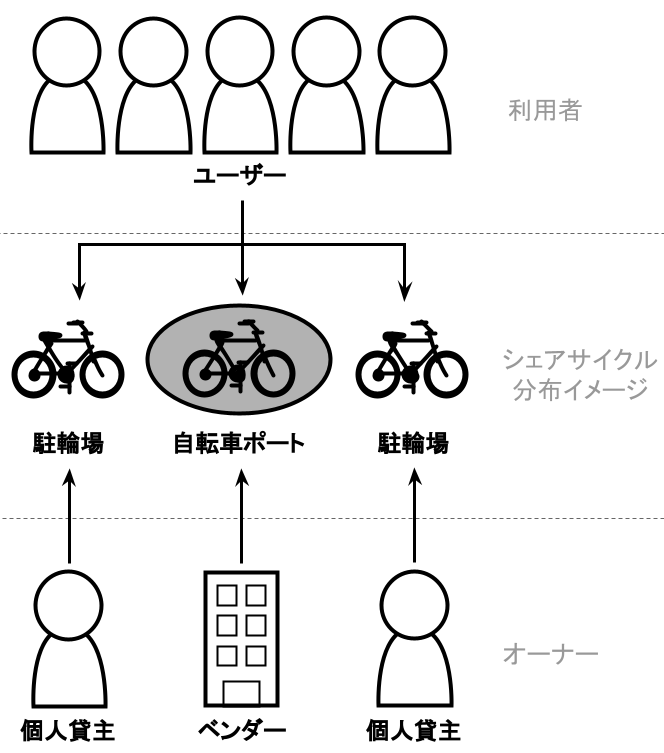
\includegraphics[scale=0.34]
            {figures/OverallImageOfSystemConfiguration.png}
            \caption{本研究において構築するシステム構成の全体像}
            \label{fig:本研究において構築するシステム構成の全体像}
          \end{figure}
          
          \begin{figure}[htbp]
            \centering
            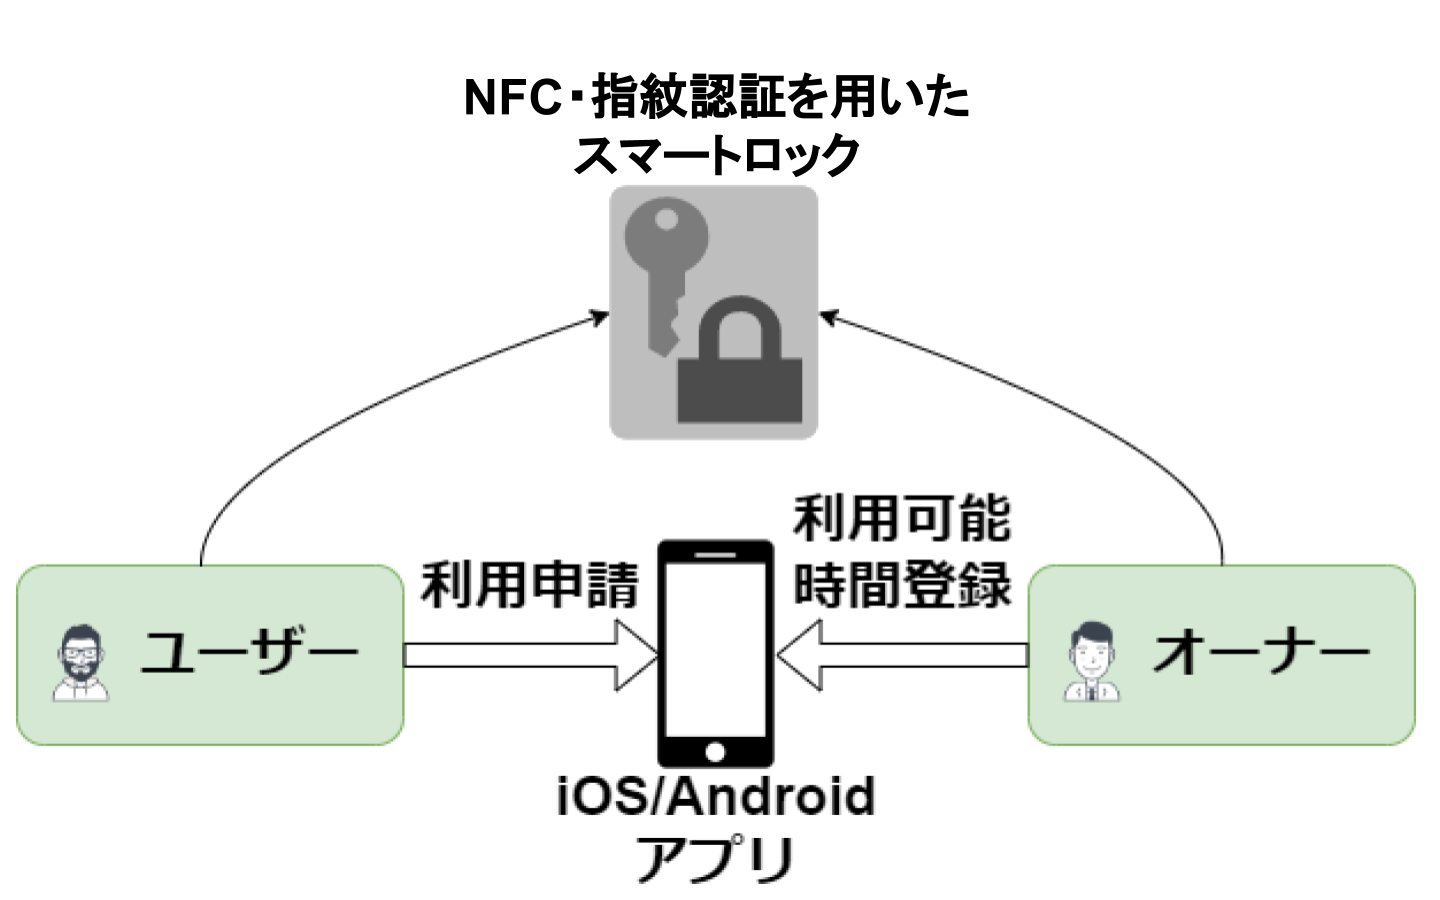
\includegraphics[scale=0.15]
            {figures/howToUse.png}
            \caption{想定するシステム利用手順概要図}
            \label{fig:想定するシステム利用手順概要図}
          \end{figure}
      
      \subsubsection{データフローの設計(\textcolor{green}{100\%})}
        \label{sec:データフローの設計}
          \par $\Box$ ER図・データの型についての話・データ保護についての話・データフロー設計において、システムのパフォーマンスを向上させるための工夫(キャッシュの利用、データの非同期処理、バッチ処理)・データ冗長性の排除(正規化、データの一元管理)
          \par データフロー設計とは,システムやアプリケーション内におけるデータの流れを視覚化し,設計するプロセスを意味する.データがどのように生成され,そのデータをどのように転送及び処理を行い,結果を格納し,さらに格納したデータをどのように使用するかを明確にするための重要な設計手法である.本研究にて構築するシステムで扱うデータの流れをデータフロー図を用いて簡潔にまとめる.なお,データフロー図には「レベル」の概念が存在し,レベルの数値が大きければ大きいほどデータフローが細分化され,システムの内のデータの流れがより具体的に表現される.一方で,レベルの数値が小さいければ小さいほどデータの流れが抽象的に表現される.
          \par レベル0のデータフロー図を図\ref{fig:レベル0のデータフロー図}の通りに表現する.レベル0では,システム全体の流れを最も抽象度高く簡略化して表現する.外部エンティティとして自転車を利用する自転車ユーザと自転車の提供者となる自転車オーナに限定し,自転車割り当てプロセスを介して自転車ユーザには割り当てられた自転車を,自転車オーナにはその結果を通知するフローを表している.
          \par レベル1のデータフロー図を図\ref{fig:レベル1のデータフロー図}の通りに表現する.レベル1では,より詳細に主要なプロセスやサブシステムを図示している.自転車ユーザからのリクエストは該当するデータベースへ一時的にストックされ,任意の時間幅でリクエストのバッチを取得する.自転車オーナは自転車登録プロセスを介して該当のデータベースへ自転車を登録し,リクエストバッチの取得プロセスの結果に基づいて自転車ユーザへ自転車を割り当てる.自転車ユーザが利用を確定した場合には,自転車データベースのレコードを更新し,スマートロック認証プロセスを介してユーザが自転車を利用できる権限を与える.同時に自転車オーナにも結果を通知する.
          \par ここで利用する主要なエンティティとしてユーザエンティティ,自転車エンティティ,ユーザリクエストエンティティが挙げられる.ただし,ここでのユーザエンティティについては,システムのユーザを指しており,自転車の利用者と自転車のオーナのどちらともをエンティティとして定義している.ユーザエンティティでは,ユーザに関する情報(ユーザID・氏名・メールアドレス・ユーザステータス・オーナステータス・住所など)を保持する.自転車エンティティでは,自転車に関する情報(自転車ID・所有者ID・車種名・ステータス・位置情報など)を保持する.ユーザリクエストエンティティでは,リクエストに関する情報(利用者ID・利用開始位置情報・目的地位置情報・利用開始時間・利用終了予想時間など)を保持する.
          \par 各プロセスにおけるデータの入力や取得は原則API通信を介して行う.入力データはクエリパラメータやエンドポイントのパスに含め,出力データはJSON形式で取得する.

          \begin{figure}[htbp]
            \centering
            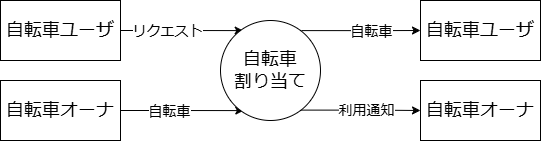
\includegraphics[scale=0.4]
            {figures/dfd-level0.drawio.png}
            \caption{レベル0のデータフロー図}
            \label{fig:レベル0のデータフロー図}
          \end{figure}

          \begin{figure*}[htbp]
            \centering
            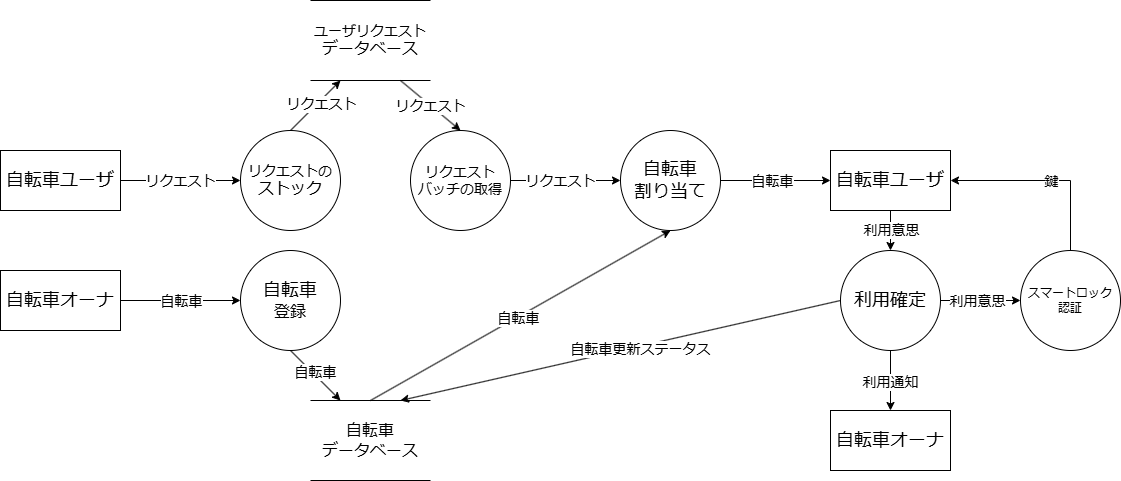
\includegraphics[scale=0.4]
            {figures/dfd-level1.drawio.png}
            \caption{レベル1のデータフロー図}
            \label{fig:レベル1のデータフロー図}
          \end{figure*}

  \subsection{スマートロックの構築(0\%)}
    \label{sec:スマートロックの構築}
      \par 
      
      \subsubsection{ハードウェア設計(\textcolor{green}{100\%})}
        \label{sec:ハードウェア設計}
          \par CtoCのシェアサイクルサービスにおいて,自転車に取り付けるスマートロックがここで指しているハードウェアである.ハードウェアは自転車の物理的な管理や盗難などのセキュリティ対策として非常に重要な役割を担っている.しかし,本研究ではハードウェアに関しては深入りせず,最終的な動作の確認のためのプロトタイプとして位置付ける.
          \par 最もハードウェアのコアとなるユーザの認証方法についてはNFC(Near Field Communication)による認証と指紋による認証の2つのアプローチを設計する.
          \par NFCによる認証をベースとした自転車のスマートロックシステムの概要を図\ref{fig:NFC認証をベースとしたスマートロックの概要図}に示す.NFCとは近距離無線通信を意味し,電子機器間の数センチメートル範囲内で発生する電磁誘導に起因してそれらの機器間の通信を可能とする\scalebox{0.7}{\cite{al2012near}}.そのNFC技術が用いられているNFCタグをスマートロックと連携することによって自転車の鍵を解錠する仕組みを構築する.想定する具体的な認証手順としては,まず,NFCを用いた自転車の鍵を自転車のオーナが自身の自転車に取り付け,別途用意するアプリケーション上でユーザが利用可能な時間を予め設定しておく.次に,ユーザは,利用したいタイミングでそのアプリケーションから利用したい希望の時間帯とマッチする自転車を探し出し,利用申請する.自転車の鍵にはNFCの他,マイコンやサーボモータを組み込み,スマートフォンがNFCにかざされ,認証されるとサーボモータが回転し,解錠する.
          \par 解錠する際のデータフローとしては,主にBlynkとIFTTTと呼ばれる2つの外部アプリケーションと連携して自転車の鍵に組み込まれているESP32マイコンと通信する.解錠する場合と施錠する場合で呼び出すIFTTT APIが異なるため,それぞれの処理を実施するためのNFCタグを別で2枚準備する.それぞれのアプリケーションの詳細や実装については\ref{sec:組み込みソフトウェアの開発}及び\ref{sec:スマートロックの構築}にて後述する.
          \par 指紋による認証をベースとした自転車のスマートロックシステムの概要を図\ref{fig:指紋認証をベースとしたスマートロックの概要図}に示す.多くの指紋認証センサにおけるセンサモジュール内部は図\ref{fig:指紋認証をベースとしたスマートロックの概要図}に示すようにセキュアに指紋情報を管理するため,その指紋認証センサを1つのモジュールとして指紋の登録や保存,認証といった一連の動作が指紋認証センサ内で完結するように組み込まれている.つまり,指紋認証センサにかざした指の指紋が,既に登録されている指紋かどうかを判定し,その結果のみが戻り値として通信される.そのため,認証結果としてマイコンが指紋認証センサから受け取る値は真偽値のみであるため,生体認証情報の漏洩リスクに関してはある程度担保されている.
          \par ESP32マイコンによる解錠処理では,指紋認証センサから取得した真偽値を元に自転車の鍵に組み込まれたサーボモータを回転させて解錠するか否かを処理する.前述した通り,NFCによる認証を行う場合は解錠する場合と施錠する場合でそれぞれのNFCタグを用意し,処理を分けることができていたが,指紋による認証の場合,1つの指紋認証センサで解錠処理と施錠処理を分けることができず,また,それぞれの処理のために2つの指紋認証センサを準備することも現実的ではないため,時間差でサーボモータが元の位置に戻り,いつでも施錠することができる状態となるようにする.

          \begin{figure}[htbp]
            \centering
            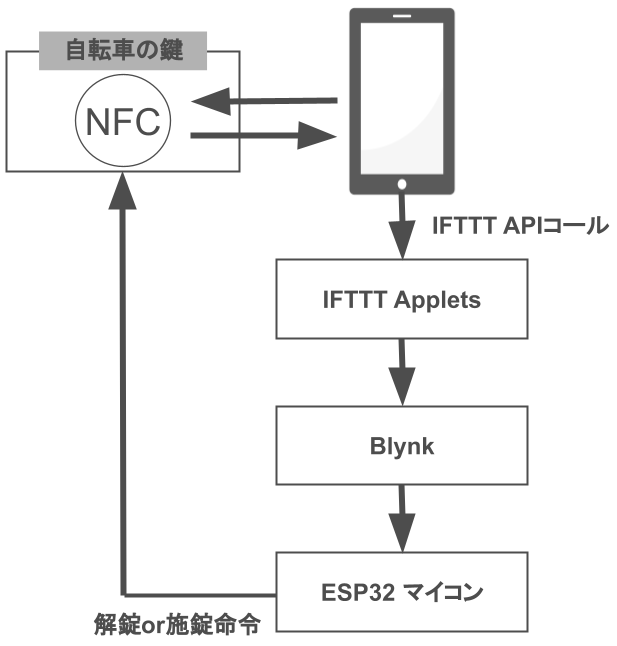
\includegraphics[scale=0.36]
            {figures/overallImageOfNfcUnlock.png}
            \caption{NFC認証をベースとしたスマートロックの概要図}
            \label{fig:NFC認証をベースとしたスマートロックの概要図}
          \end{figure}
          
          \begin{figure}[htbp]
            \centering
            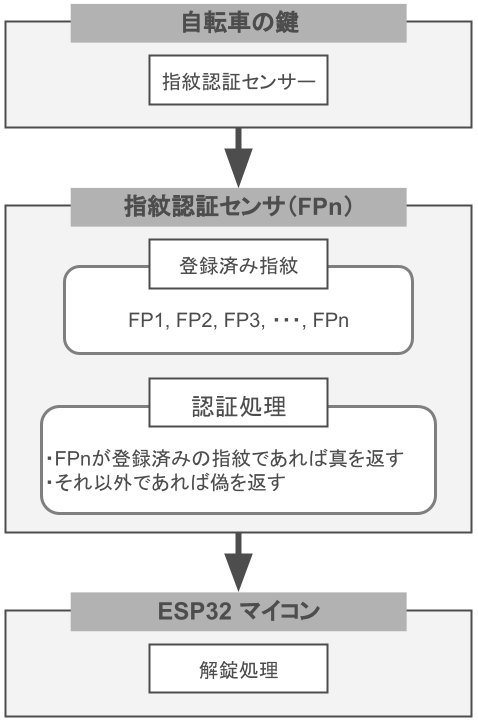
\includegraphics[scale=0.46]
            {figures/overallImageOfFingerprintUnlock.png}
            \caption{指紋認証をベースとしたスマートロックの概要図}
            \label{fig:指紋認証をベースとしたスマートロックの概要図}
          \end{figure}
          
          
      \subsubsection{組み込みソフトウェアの開発(0\%)}
        \label{sec:組み込みソフトウェアの開発}
          \par
          
      \subsubsection{通信プロトコルの選定(0\%)}
        \label{sec:通信プロトコルの選定}
          \par
          
  \subsection{マッチングモデルの設計(0\%)}
    \label{sec:マッチングモデルの設計}
      \par

      \subsubsection{数理最適化モデルの定式化(\textcolor{green}{100\%})}
        \label{sec:数理最適化モデルの定式化}
          \par $\Box$ 変数や制約の数、計算複雑性について触れる。
          \par シェアサイクルサービスをCtoC化することによる特徴として,サービスを提供するために大量の自転車を予め確保する必要性がなく,個人が所有している未使用の自転車を有効活用することができる点や,都市部と地方で設置数に偏りが生じやすいポートに依存せず,ポートがない場所でも乗り捨てが可能となり,移動自由度の向上が期待できる点が挙げられる.また,自転車保有者側の観点においても,自転車を利用していない期間にそれをユーザに貸し出すことで,自身のリソースを有効活用できると捉えることもできる.一方で,ユーザに対して適切な自転車が割り当てられない場合や,既存のシェアサイクルシステムのようにユーザが好みの自転車を自由に選択することができる状況下においては,乗り捨てられた自転車とその保有者との位置関係が未知数となり,自転車を再配置する際に多くのコストを要することが想定される.
          
          \par そこで,個人所有の自転車を効率的にシェアし,乗り捨て可能なシェアサイクルシステムを実現するため,数理最適化ベースの自転車割り当てモデルを設計し,構築する.ユーザに自転車を割り当てるアルゴリズムを数式としてモデル化し,それに基づいて自転車割り当て処理が実行されるため,乗り捨て可能な個人所有自転車のシェアリングにおいて的確な割り当て結果を得ることが期待される.
          
          \par モデルの構築においては,整数計画法によるアルゴリズムを軸とする.
          
          \par 整数計画法は,一部または全ての決定変数が整数値のみをとるように制約された線形計画法である\scalebox{0.7}{\cite{wolsey2020integer}}.一方で,線形計画法では,変数は整数値以外も取ることができる.そのため,本研究でアプローチしているような整数計画問題を線形計画法を用いたプロセスで処理しようとすると,線形計画法による解が整数ではない場合,丸めた解が実行不可能または最適ではない可能性がある\scalebox{0.7}{\cite{hooker2024integer}}.整数計画法では,決定変数が整数であるべき多くの現実世界の状況をモデル化するのに役立つ\scalebox{0.7}{\cite{gomory1960integer}}.これらの観点を踏まえ,個人所有の自転車をユーザに割り当てる問題では,決定変数が「割り当てるか否か」のバイナリ変数であるべき問題であることより,整数計画法を用いたアルゴリズムを構築する.
          
          \par 前提条件として,本モデルが数理最適化ベースであることの利点を最大限活用するため,ユーザから自転車割り当てシステムに対するリクエストは1分間ストックし,ストックされたリクエストデータに対して毎分バッチ処理を実行する.また,シェアリングの対象は個人所有の自転車とし,ユーザ体験の観点において,移動自由度を向上させることを目的としてドックレスで乗り捨て可能なシステムを想定する.なお,乗り捨てによる自転車の不法駐輪等の法的な課題に関してはここでは考慮せず,あくまで自転車の割り当て問題として切り分けてモデリングする.
          
          \par 定式化で用いる集合やパラメータ,決定変数のそれぞれの記号と概説を表\ref{tab:記号の概説}に示す.ユーザリクエストの集合を$R$,シェアリングされる自転車の集合を$B$とする.ユーザ$r (r \in R)$に自転車$b (b \in B)$が割り当てられる前の初期状態として,ユーザとユーザがリクエストした時点での自転車の距離関係を表すパラメータを距離行列$d^{\text{init}}_{b,r}$とする.ユーザ$r (r \in R)$に自転車$b (b \in B)$が割り当てられ,ユーザが割り当てられた自転車に乗って移動したと仮定した場合のその後の自転車の位置と自転車の所有者までの距離関係を表すパラメータを距離行列$d_{b,r}$とする.
          
          \begin{table}[htbp]
            \caption{記号の概説}
            \label{tab:記号の概説}
            \centering
            \begin{tabular}{c p{6cm}}
              \hline 
              記号 & 説明 \\
              \hline
              $R$ & ユーザリクエストの集合 \\
              $B$ & シェアリングされる自転車の集合 \\
              $d^{\text{init}}_{b,r}$ & ユーザ $r(r \in R)$ と自転車 $b(b \in B)$ の割り当て前の距離行列\\
              $d_{b,r}$ & ユーザ $r (r \in R)$ に自転車 $b (b \in B)$ が割り当てられて移動した後の距離行列 \\
              $x_{b,r}$ & ユーザ $r (r \in R)$ に自転車 $b (b \in B)$ が割り当てられたか否かの二値変数行列 \\
              \hline
            \end{tabular}
          \end{table}
          
          \par 決定変数については,ユーザ$r (r \in R)$に自転車$b (b \in B)$が割り当てられたか否かの二値変数行列$x_{b,r}$とする.ユーザ$r$が自転車$b$を利用する場合に1,そうでなければ0のバイナリ値を持つ.
          
          \par 目的関数は\ref{equ:目的関数}式の通りに定義する.
          
          \begin{equation}\label{equ:目的関数}
            \min \left( \sum_{b \in B}\sum_{r \in R}d_{b,r}x_{b,r} - \alpha\sum_{b \in B}\sum_{r \in R}x_{b,r} \right)
          \end{equation}
          
          \begin{equation}\label{equ:移動後の距離最小化}
            \min \left( \sum_{b \in B}\sum_{r \in R}d_{b,r}x_{b,r} \right)
          \end{equation}
          
          \begin{equation}\label{equ:割り当て成功率最大化}
            \max \left(\sum_{b \in B}\sum_{r \in R}x_{b,r} \right)
          \end{equation}
          
          \par 第1項の部分については,\ref{equ:移動後の距離最小化}式に示す通り,ユーザが割り当てられた自転車に乗って移動した後の自転車とその自転車の所有者までの距離を最小化する.例えば,あるユーザからのリクエストがあった場合,そのユーザの現在地と目的地,リクエストされた時点での自転車とその自転車の所有者までの位置関係が図\ref{fig:ユーザと自転車の初期位置とリクエスト方向}の状態であったとする.なお,自転車の位置は自転車のアイコンで,自転車の所有者の位置は家のアイコンで表し,所有関係は色に対応している.この場合,\ref{equ:移動後の距離最小化}式に従うと,ユーザには緑色の自転車が割り当てられる.ユーザが移動した直後の状態が図\ref{fig:自転車割り当て・移動後の位置関係}に示す通りとなり,橙色の自転車が割り当てられた場合と比較して,点線で示した自転車とその自転車の所有者との距離の総和が小さくなる.
          
          \begin{figure}[htbp]
            \centering
            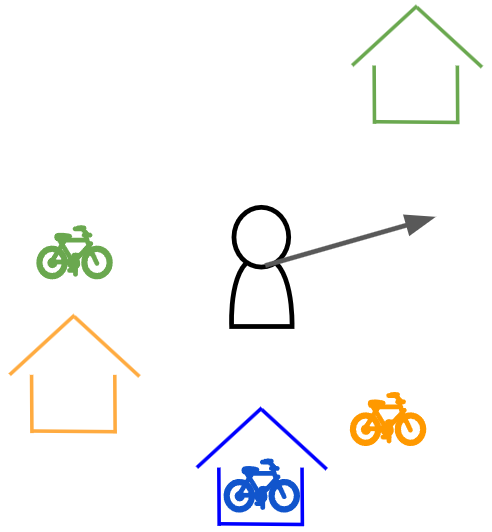
\includegraphics[scale=0.6]
            {figures/subjectFunction1-0.png}
            \caption{ユーザと自転車の初期位置とリクエスト方向}
            \label{fig:ユーザと自転車の初期位置とリクエスト方向}
          \end{figure}
          \begin{figure}[htbp]
            \centering
            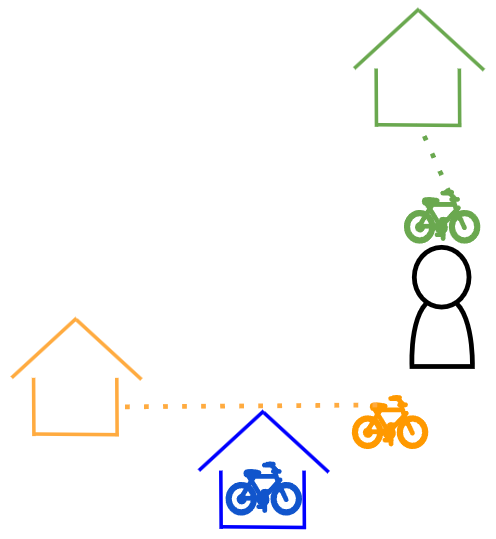
\includegraphics[scale=0.6]
            {figures/subjectFunction1-1.png}
            \caption{自転車割り当て・移動後の位置関係}
            \label{fig:自転車割り当て・移動後の位置関係}
          \end{figure}
          
          \par 第2項の部分については,\ref{equ:割り当て成功率最大化}式に示す通り,可能な限り多くのユーザに自転車を割り当てる最大化を行う.\ref{equ:移動後の距離最小化}式のみを目的関数として定義した場合,全ての自転車が所有者の手元にあるような極端な状況ではユーザに自転車を一切割り当てない選択をすることが,割り当て移動後の自転車とその自転車の所有者までの距離が最小化される結果となり,最適と判断されてしまう.サービスとしてもユーザに自転車が割り当てられることで初めて機能するため,\ref{equ:割り当て成功率最大化}式を目的関数の一部としている.
          
          \par なお,\ref{equ:移動後の距離最小化}式と\ref{equ:割り当て成功率最大化}式は最小化と最大化のトレードオフの関係にあるため,\ref{equ:割り当て成功率最大化}式に対してトレードオフの調整を行う重み$\alpha$を掛け合わせ,このトレードオフの最適値を探る.ただし,$\alpha$は非負であることを保証し,指定が無い場合は$\alpha=1$とする.\ref{equ:割り当て成功率最大化}式に対して$-\alpha$を掛け合わせることで,目的関数全体として最小化を行う.
          
          \par 制約条件は\ref{equ:半径制約}式から\ref{equ:人対自転車}式の通りに定義する.
          
          \begin{equation}\label{equ:半径制約}
            x_{b, r} \leq \mathbb{I}(d^{\text{init}}_{b, r} \leq 250), \forall b \in B, \, \forall r \in R
          \end{equation}
          
          \begin{equation}\label{equ:自転車対人}
            \sum_{r \in R}x_{b,r} \leq 1, \forall b \in B
          \end{equation}
          
          \begin{equation}\label{equ:人対自転車}
            \sum_{b \in B}x_{b,r} \leq 1, \forall r \in R
          \end{equation}
          
          \par \ref{equ:半径制約}式は,ユーザから半径250m以内の自転車のみを割り当てる制約を意味する.図\ref{equ:半径制約}に示すように,ユーザから半径250mの範囲外に位置する自転車は割り当ての対象外となる.\ref{equ:自転車対人}式は,図\ref{fig:自転車に割り当てられるユーザは1人以下}に示すように,自転車に割り当てられるユーザは1人以下であることを定義し,\ref{equ:人対自転車}式は,図\ref{fig:ユーザに割り当てられる自転車は1台以下}に示すように,ユーザに割り当てられる自転車は1台以下であることを定義する.これらの制約条件を設けることによって,ユーザから遠く離れた場所に位置する自転車の割り当てや,利用する自転車がユーザ同士で重複して割り当てられること,ユーザが複数台の自転車を利用して移動することを防ぐ.
          
          \begin{figure}[htbp]
            \centering
            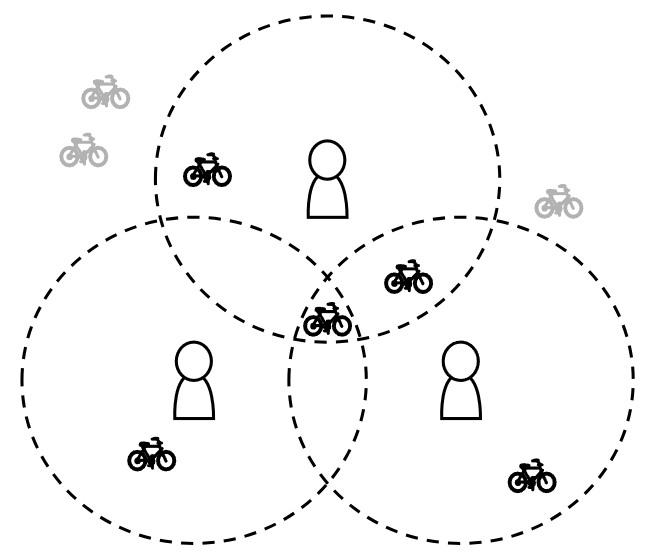
\includegraphics[scale=0.45]
            {figures/objectFunction1.png}
            \caption{割り当て許容距離に含まれている自転車の状態}
            \label{fig:割り当て許容距離に含まれている自転車の状態}
          \end{figure}
          
          \begin{figure}[htbp]
            \centering
            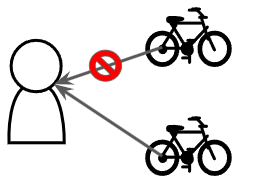
\includegraphics[scale=1.18]
            {figures/objectFunction2.png}
            \caption{自転車に割り当てられるユーザは1人以下}
            \label{fig:自転車に割り当てられるユーザは1人以下}
          \end{figure}
          
          \begin{figure}[htbp]
            \centering
            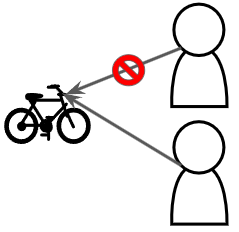
\includegraphics[scale=1.2]
            {figures/objectFunction3.png}
            \caption{ユーザに割り当てられる自転車は1台以下}
            \label{fig:ユーザに割り当てられる自転車は1台以下}
          \end{figure}

      \subsubsection{機械学習モデルの設計(0\%)}
        \label{sec:machine_learning_model_design}
          \par

  \subsection{APIの設計方針(\textcolor{green}{100\%})}
    \label{sec:APIの設計方針}
      \par 本研究において構築したスマートロックやマッチングモデルを1つの一貫したシステムとして完結させるためにはそれぞれのモジュールのインターフェースとなるAPIが必要不可欠である.APIの役割と重要性については\ref{sec:コア技術の活用}節にて述べた.ここではそのAPIを設計するにあたって,APIの機能要件の定義やセキュリティに関わる考慮事項などをまとめる.
      
      \subsubsection{API機能要件の定義と設計(\textcolor{green}{100\%})}
        \label{sec:API機能要件の定義と設計}
          \par API(Application Programming Interface)はアプリケーションとプログラミング的なやり取りを可能とするインターフェイスである.標準プロトコルを用いて文書化され,クライアントとサーバーの両方がそのAPIドキュメントに従っている限り,通信は期待通りに実行される.詳細は\ref{sec:コア技術の活用}節にて論じた.本研究において構築する自転車割り当てモデルをアプリケーション上のサービスとしてユーザに価値提供するためにAPIを利用する.
          \par APIの設計においてはREST APIの設計原則に準拠して設計する.特に,RESTの設計原則ではステートレスなアーキテクチャであることが挙げられており,これによってスケーラビリティや信頼性の向上が期待できる.需要を予測することが難しいCtoCシェアサイクルサービスにおいて,ニーズに合わせたサーバー処理が求められることから適切であると判断した.また,自転車のスマートロックなどのIoTデバイスとの連携においても,軽量であり様々なIoTデバイスとの通信に広く利用されている点も選定基準の1つである.
          \par \ref{sec:システム要件の定義}節にて定義したシステム要件から導出される,APIが提供するべき具体的な機能として,マイクロサービス単位で換算すると5つである.自転車割り当てサービス・自転車利用サービス・ユーザ管理サービス・自転車管理サービス・スマートロック操作サービスである.なお,マイクロサービスとは,マイクロサービス分野をリードする著者の1人であるSam Newman氏によると「一体となって動作する,小規模な自律的なサービス」と定義されている\scalebox{0.7}{\cite{newman2021BuildingMicroservices}}.また,James Lewis氏とMartin Fowler氏の記事によると,「1つのアプリケーションを一連の小さなサービスの組み合わせとして開発するアプローチ.これらのサービスはそれぞれの独自のプロセスで実行され,軽量なメカニズム(多くの場合はHTTPリソースAPI)を用いて通信する」と定義されている\scalebox{0.7}{\cite{Microservices}}.これらより,システムの各コンポーネントを個別にデプロイ可能なサービスとしてカウントできる単位をマイクロサービスとして定義する.
          \par 上記のサービスに基づき,必要なAPI機能となるエンドポイントを表\ref{tab:Bikeying API エンドポイント一覧}に一覧化する.なお,本研究にて構築するAPIをBikeying APIと命名し,以後適宜その名称を用いる.自転車割り当てサービスでは,本研究で構築する自転車割り当てモデルのメイン処理を実装し,ユーザのリクエストに基づいた最適な自転車を割り当て,レスポンスする.自転車利用サービスは,実際にユーザが自転車を検索し,予約する際に,クライアントと自転車割り当てサービスとのインターフェイスとしての役割を果たす.ユーザのリクエストをある一定期間ストックする場合などに効果を発揮する.自転車管理サービス及びユーザ管理サービスでは,それぞれ自転車やユーザの追加や削除,ステータスの管理を行う責務を果たす.スマートロック操作サービスでは,自転車割り当てサービスや自転車利用サービスの結果に基づき,対象のスマートロックの解錠・施錠をAPI経由で制御できるようにする.
          \par ここで定義したBikeying APIのそれぞれのマイクロサービス間の基本的な関連性と,クライアントやIoTスマートロックとのインターフェースとしての立ち位置の概要を図\ref{fig:サービス間とインターフェースの関連}に示す.自転車利用サービスを軸として,クライアントからのリクエストを各々の責務を果たすマイクロサービスへと分散し,レスポンスする.IoTスマートロックの操作が必要となる場合は,図\ref{fig:サービス間とインターフェースの関連}に示す通り,スマートロック操作サービスがそのインターフェースとしての役割を果たす.

          \begin{table*}[t]
            \caption{Bikeying API エンドポイント一覧}
            \label{tab:Bikeying API エンドポイント一覧}
            \centering
            \begin{tabular}{|p{3.5cm}|l|p{5cm}|l|l|} \hline
              マイクロサービス & エンドポイント & 説明 & HTTPメソッド & 認証 \\ \hline
              自転車管理サービス & \url{/bikes} & 自転車の現在の利用ステータスを取得する & GET & 必須 \\ \cline{2-5}
              & \url{/bikes} & 自転車の現在の利用ステータスを更新する & PUT & 必須 \\ \cline{2-5}
              & \url{/bikes} & シェアリング可能な自転車を追加する & POST & 必須 \\ \cline{2-5}
              & \url{/bikes} & 自転車をシェアリングの対象から削除する & DELETE & 必須 \\ \hline
              自転車割り当てサービス & \url{/bikes/dispatch} & ストックされたリクエストから最適な自転車を割り当てる & GET & 必須 \\ \hline
              自転車利用サービス & \url{/bikes/requests} & ユーザの現在地座標などの条件に基づいたリクエストをストックする & POST & 必須 \\ \cline{2-5}
              & \url{/bikes/reserve} & 特定の自転車の利用を確定・予約する & POST & 必須 \\ \hline
              ユーザ管理サービス & \url{/users/signup} & 新規ユーザ登録 & POST & なし \\ \cline{2-5}
              & \url{/users/login} & ユーザのログイン処理 & POST & なし \\ \cline{2-5}
              & \url{/users/logout} & ユーザのログアウト処理 & POST & 必須 \\ \cline{2-5}
              & \url{/users/{userId}} & ユーザのプロフィール情報を取得する & GET & 必須 \\ \cline{2-5}
              & \url{/users/{userId}} & ユーザのプロフィール情報を更新する & PUT & 必須 \\ \hline
              スマートロック操作サービス & \url{/{lockId}/unlock} & 指定されたスマートロックを解錠する & POST & 必須 \\ \cline{2-5}
              & \url{/{lockId}/lock} & 指定されたスマートロックを施錠する & POST & 必須 \\ \cline{2-5}
              & \url{/{lockId}/status} & スマートロックの状態を取得する & GET & 必須 \\ \hline
            \end{tabular}
          \end{table*}

          \begin{figure}[htbp]
            \centering
            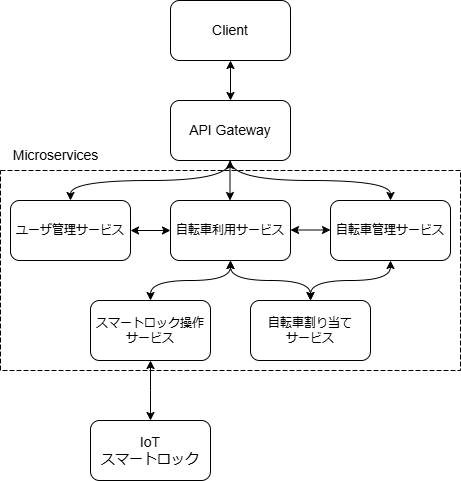
\includegraphics[scale=0.49]
            {figures/microservice-architecture.png}
            \caption{サービス間とインターフェースの関連}
            \label{fig:サービス間とインターフェースの関連}
          \end{figure}

      \subsubsection{セキュリティと認証の設計(\textcolor{green}{100\%})}
        \label{sec:セキュリティと認証の設計}
          \par $\Box$ 認証シーケンス図作成したい
          \par APIのセキュリティを考える上で認証及び認可の設計は,システムの信頼性とデータ保護を確保するために非常に重要であり,避けて通ることはできない.不適切なセキュリティ設計は,データの漏洩や不正アクセスなどの深刻な問題を引き起こす可能性がある.実際にAPI認証システムの脆弱性による被害が発生してる事例が存在する.例として,本研究と似通ったライドシェアサービスを展開しているUber社の事例を紹介する.2016年に,Uber社の開発者用APIキーがGitHubに公開されたことをきっかけに,Uber社が利用してる第三者機関のクラウドベースのサーバーにてユーザデータに不正なアクセスがあったことが発覚しした.APIキーを利用した攻撃により,日本でもおよそ10万人の乗客及びドライバに関する情報が漏洩したとされている\scalebox{0.7}{\cite{uber2016dataincident}}.そのため,本項では堅牢なシステム構築の重要な要素となるAPIにおける認証および認可を設計する.
          \par 認証とはAPIを利用しようとしてるユーザやアプリケーションが「誰であるか」を確認するプロセスである.これは「本人確認」に相当し,ユーザがAPIにアクセスするために提供したAPIキーやトークンなどが正しいかを判定する.一方で,認可とは認証済みのユーザやアプリケーションが「何をすることを許可されているか」を制御するプロセスである.これは「権限管理」に相当し,認証後にそのユーザが特定のリソースや機能へのアクセスが許可されているかを判定する.
          \par APIの認証で用いられる重要なプロトコルとしてはOAuth(Open Authrization)やOpenID Connect,JWT(Json Web Token)の3つが挙げられる.
          \par OAuthは,OAuthプロバイダーを通して認証と認可を行う,アクセス委任の標準プロトコルである\scalebox{0.7}{\cite{oauth}}.一般に,アクセスはトークンの発行により許可され,そのトークンを用いることで外部サービスとの連携が容易である点が特徴である.
          \par OpenID Connectは,OAuthプロトコルをベースとして構築された認証プロトコルであり,このプロトコルを用いることで,クライアントは認可サーバーの認証結果に基づいてエンドユーザを検証することができる.また,同時にエンドユーザに必要なプロフィール情報などもRESTfulな形式で取得することが可能となる\scalebox{0.7}{\cite{openidconnectjapan}}.
          \par JWTは,認証や認可,セキュリティを容易に実装するために当事者間でデータを交換するための軽量な手段となるJSONドキュメントを表すトークンである\scalebox{0.7}{\cite{mahindraka2020insights}}.JWTはプライベートシークレットもしくは暗号鍵を用いて署名され,そのドキュメントにはトークンの発行者やその対象,有効期限などの情報を含んでいる.これはOAuthにおいてもOpenID Connectにおいてもユーザのアクセスの検証として用いられている.
          \par 本研究で構築するAPIの認証及び認可においては,マイクロサービスアーキテクチャを採用しており,サービス間での認証と認可に適している点と,簡易的な認証基盤を設計し構築に要する時間的コストを削減する点を鑑みてこれらの認証プロトコルを用いて構築する.
          \par そこで,JWTのペイロードのクレームに含まれているそれぞれの項目の設定値を定義する.JWTの発行者を識別するためのiss(issuer)にはBikeying APIのドメイン及びそのURLを定義する.サーバーにリクエストを送信するユーザを識別するためのsub(subject)には適当なuuidを定義する.JWTが意図する受信者を識別するためのaud(audience)にはローカルホスト環境で立ち上げるURLを定義する.JWTが発行された日時のタイムスタンプであるiat(issued at time)には現在時刻を定義する.JWTの有効期限を指定するexp(expiration time)には現在時刻から24時間後の時刻を定義し,このトークンの有効期限は24時間とする.認証プロトコルにはOpenID Connectを用いるため,scope(scope value)にその旨を定義する.実際に定義したpayloadはListing \ref{list:JWTペイロード}の通りである.
          \par APIサーバーに認可を追加するため,生成したJWTを利用してAuthミドルウェアを構築する.悪意のあるユーザに情報を与えないためにも,認証及び認可に失敗した場合は403レスポンスではなく404レスポンスを返すこととする.ただし,Swagger UIで構築しているAPI仕様書やOpenAPIのJSONエンドポイントに対して認可を設定すると全てのAPIのエンドユーザが利用できなくなる場合も想定されるため,この2点については認証及び認可の処理を通らないよう考慮する.
          \par さらにセキュリティの観点において,CORS(Cross-Origin Resource Sharing)ミドルウェアも追加する.CORSとは異なるドメインやプロトコル,ポートからリソースにアクセスすることを許可するメカニズムである.通常は異なるオリジンからのアクセスは制限されるが,指定されたHTTPヘッダーを使用することで制限を緩和し,異なるオリジンを跨いだリソースの共有を可能とする\scalebox{0.7}{\cite{dresen2020corsica}}.

\lstset{
  identifierstyle={\small},
  commentstyle={\smallitshape},
  keywordstyle={\small\bfseries},
  ndkeywordstyle={\small},
  stringstyle={\small\ttfamily},
  frame={tb},
  breaklines=true,
  columns=[l]{fullflexible},
  numberstyle={\scriptsize},
  stepnumber=1,
  lineskip=-0.5ex
}
\begin{lstlisting}[caption={JWTペイロード}, label={list:JWTペイロード}, basicstyle=\ttfamily\footnotesize]
payload = {
  "iss": "https://auth.bikeying.com",
  "sub": "12e49b07-5ff3-4e2d-bfdf-6ac315ce5f33",
  "aud": "http://127.0.0.1:8000/bikes",
  "iat": now.timestamp(),
  "exp": (now + timedelta(hours=24)).timestamp(),
  "scope": "openid",
}
\end{lstlisting}
  % 第4章
    \clearpage
    \newpage
    % 第5章
\section{実装(\textcolor{orange}{14\%})}
  \label{sec:実装}
    \par
  
  \subsection{スマートロックの実装(0\%)}
    \label{sec:スマートロックの実装}
      \par
  
      \subsubsection{プロトタイプ作成(0\%)}
        \label{sec:プロトタイプ作成}
          \par
          
      \subsubsection{動作確認(0\%)}
        \label{sec:動作確認}
          \par
          
  \subsection{数理最適化モデルの実装(0\%)}
    \label{sec:数理最適化モデルの実装}
      \par
      
      \subsubsection{ソルバーの選定(\textcolor{green}{100\%}))}
        \label{sec:ソルバーの選定}
          \par ソルバーの性能は,結果の質や計算時間に大きく影響するため,自転車割り当て問題を効率的かつ正確に解くためには適切なソルバーの選定が必要不可欠である.特に,CtoCシェアサイクルシステムにおいては,リアルタイム性やスケーラビリティが求められるため,最適なソルバー選定がシステム全体のパフォーマンスを左右する.
          
          \par 本研究で扱っている自転車割り当て問題の特徴としては,整数線形計画問題として定式化される点が最大の特徴として挙げられる.他にも,変数にはバイナリ値のみが含まれ,制約条件は線形である点も特徴として挙げられる.問題の規模感としては,シェアリングの対象となる自転車の数やユーザの需要などに応じて決定変数である二値変数行列の成分の数が大規模になる可能性も考えられる.そのような状況下においても最適な自転車をユーザに割り当てる必要があるため,解の精度は高く保たれる必要がある.さらに,リアルタイム性が求めらる点も考慮すると,迅速な計算処理を継続して行う必要もある.
          
          \par そこで,ソルバーを選定するにあたって,上記の要件を満たすための観点をいくつかまとめる.まず性能面において,大規模問題でも迅速に解を求められ,効率的なメモリ管理が可能であることや,整数線形計画問題に対応していることが求められる.また,利便性の面において,無料で利用可能であることや,アルゴリズムの実装の際に用いるOR-Toolsとの互換性も求められる.なお,OR-ToolsとはGoogle社から提供されている組み合わせ最適化向けのオープンソースソフトウェアであり,非常に広範な可能性のあるソリューションの中から問題に対する最適化ソリューションを見つけ出すことをサポートする\scalebox{0.7}{\cite{OR-Tools}}.
          
          \par 具体的なソルバーの例として,CPLEXやGurobiなどが挙げられる.CPLEXはIBM社から提供されている,混合整数計画法のための分散型並列アルゴリズムと,線形計画,混合整数計画などのための柔軟で高性能な数理計画法ソルバーである\scalebox{0.7}{\cite{CPLEX}}.GurobiはGurobi社から提供されているソルバーであり,並列処理を最大限活用するよう構築され,高度なMIPヒューリスティックアルゴリズムにより実現可能解を素早く求解可能である特徴を持つ\scalebox{0.7}{\cite{Gurobi}}.しかし、これらのソルバーはオープンソースではないが故に,ライセンス費用の面における制限が懸念される.
          
          \par オープンソースソルバーの例としては,GLPKやCBCなどが挙げられる.
          
          \par GLPKはモスクワ航空大学のAndrew Makhorin氏によって開発されたソルバーである.C言語で記述されており,コマンドラインまたはAPIを介して操作可能であり,CとJavaのAPIを提供している.CPLEXのような商用ソルバーと比較するとGLPKの速度は劣るものの,線形計画問題に対して有効なソルバーである\scalebox{0.7}{\cite{gearhart2013comparison}}.
          
          \par CBCはJohn Forrest氏らによって開発された,COIN-OR線形計画法を用いた混合整数計画問題を解くためのソルバーである.C++で書かれており,呼び出し可能なライブラリとしても,スタンドアロンの実行ファイルとしても利用可能である.様々なモデリングシステムやパッケージなどを通して,様々な方法で利用することができる\scalebox{0.7}{\cite{CBC}}.
          
          \par また,オープンソースソルバーの別の例としてSCIPも挙げられる.SCIPは,混合整数線形計画問題や混合整数比線形計画問題,さらには制約整数計画問題のソルバーとして設計された,制約整数計画ソルバーである\scalebox{0.7}{\cite{bolusani2024scip}}.SCIPソルバーは汎用性の高いフレームワークであり,問題のサイズを縮小する前処理や下界値を強化するカット生成,より良い上限値を与えるためのヒューリスティック解法などの機能をプラグインとして追加することができる.これによってSCIPソルバーの利用者は問題に合わせてカスタマイズし,性能を向上させることができる\scalebox{0.7}{\cite{shinano2013CIPSolver}}.一方で,SCIPを利用することの欠点としては,高機能であるが故に複雑性が高く,ある程度の学習コストを要する点や,多数のパラメータを持ち,その設定によって性能が大きく変化するため,最適なパラメータを見つけるためのチューニングが難しい場合がある.
          
          \par 上記で述べた要件やソルバーの一長一短を鑑み,本研究ではSCIPを自転車割り当てにおける整数線形計画問題のソルバーとして選定する.選定理由の最も大きなポイントとしては,オープンソースのソルバーであり,利用するにあたってライセンス関連のコストを懸念する必要が無い点である.オープンソースソルバーとしてSCIP以外に挙げたGLPKやCBCと比較して計算速度が優位である点もSCIPを選定したポイントの1つである.さらに,アルゴリズムの実装の際に用いるOR-Toolsとの互換性が高い点も選定ポイントとして挙げられる.SCIPを利用する際のデメリットとして挙げた複雑性について,OR-Toolsを併用して利用した場合,比較的シンプルにアルゴリズムを実装することが可能となるため,SCIPの長所を最大限生かした実装を行えることが期待される.
          
      \subsubsection{アルゴリズムの実装(\textcolor{green}{100\%})}
        \label{sec:アルゴリズムの実装}
          \par 本研究で提案する数理最適化ベースの自転車割り当てアルゴリズムは,単にユーザの最短距離に配置されている自転車を割り当てるわけではない.複数のリクエストをストックした上で,\ref{sec:数理最適化モデルの定式化}項で定義した目的関数や制約条件のもと,ユーザの移動後の自転車の配置が全体最適となるように割り当てることによって,CtoCシェアサイクルサービスを実現させることを目的としている.
          \par そこで,実際に\ref{sec:ソルバーの選定}項にて選定したSCIPソルバーを用いて数理最適化ベースの自転車割り当てモデルをモジュールとして実装する.実装する際にはプログラミング言語Pythonを利用する.Pythonとは,1991年にGuido van Rossum氏によって開発されたプログラミング言語であり,コードの可読性を重視した設計哲学や動的型付け言語でありコンパイルが不要である点,包括的な標準ライブラリがサポートされている点などが特徴として挙げられる\scalebox{0.7}{\cite{aboutPython}}.その他,主要なライブラリ及びパッケージとしてSciPyやNumpy,Pandasなどを用い,開発環境としてGoogle Colaboratoryを利用する.
          \par ユーザリクエストをストックするために定義されるある時間幅に対して処理を実行するアルゴリズム全体のフローチャートは図\ref{fig:自転車割り当てアルゴリズムのフローチャート}で示す通りである.ただし,割り当てモデルクラスをインスタンス化する際のパラメータとして,データフレーム型の地理情報データとシェアリングされる自転車データ$B$を指定する.そうすることによって,指定された地域の特性や利用可能な自転車の数,及びステータスに対して柔軟に対応可能となる.なお,ここで用いる記号で説明を省略している場合は,表\ref{tab:記号の概説}の通りとする.
          \par 距離行列の生成では,入力されるリクエストデータや自転車のステータスから自転車の現在地や自転車の所有者までの位置,ユーザの現在地などの位置情報を取得し, 測地線距離を用いてそれぞれの対象間の距離を計算し,行列として値を格納する.測地線距離とはリーマン多様体上の2点間の最短経路の長さとして定義\scalebox{0.7}{\cite{shuvo2024geodesic}}され,空間の曲率を考慮した距離を算出する.さらに,距離のスケールを統一するため,生成した距離行列に対してデータの平均が0,標準偏差が1になるよう正規化を実施する.これにより,モデルクラスをインスタンス化する際の地理情報データに依存せず,一貫性を持ったパラメータの調整を行うことができる.
          \par 利用可能な自転車$B_{\text{able}}$は二値行列であり,リクエストされた時刻とシェアリング対象自転車の集合$B$の貸し出し終了日時カラムの値を元に生成される.貸し出し終了日時がNullまたはリクエストされた時刻より過去である自転車は現在利用可能であると判定され1を格納し,それ以外の場合は0を格納する.
          \par データの取得・整形後に数理最適化を実行し,自転車とユーザの割り当て解が存在するか否かを確認する.解が存在しない場合は処理を終了する.解が存在する場合は,その割り当て解を返し,さらに,シェアリング対象自転車の集合$B$の割り当てられたそれぞれの自転車に対して貸し出し終了日時カラムの値をユーザリクエストの情報を元に更新する.以降,シェアリング対象自転車の集合$B$を取得する際に,更新された自転車のステータスを元に$B_{\text{able}}$の取得処理が繰り返される.
          \par より大規模なリクエストデータ及び自転車データに対して自転車割り当てアルゴリズムを適用する場合,計算処理に多くのコストを要し,レスポンスまでの待機時間が大幅に上昇する場合がある.レスポンスまでの時間が増大するとユーザ体験は著しく低下し兼ねない.そのため,必要に応じてPythonによるGPU高速計算のためのオープンソースの配列ライブラリCuPyを利用する.CuPyのインターフェースはNumPyと高い互換性を持ち,NumPy配列を定義・利用している箇所をCuPyに置き換えるだけでGPUで並列処理を適切に実行することができ,レスポンスまでの時間を縮小することができる\scalebox{0.7}{\cite{CuPy}}.
          \par エラーハンドリングとして,モデルに入力される値に対しての例外処理を実装する.例えば,インスタンス化する際に入力されるデータフレーム型の地理情報データの経度・緯度カラムに有効な値が格納されているかや,リクエストデータが有効なデータフレームであるかなどの観点が挙げられる.条件分岐による例外出力や随時デバッグ出力にて確認できるよう構築する.

          \begin{figure}[htbp]
            \centering
            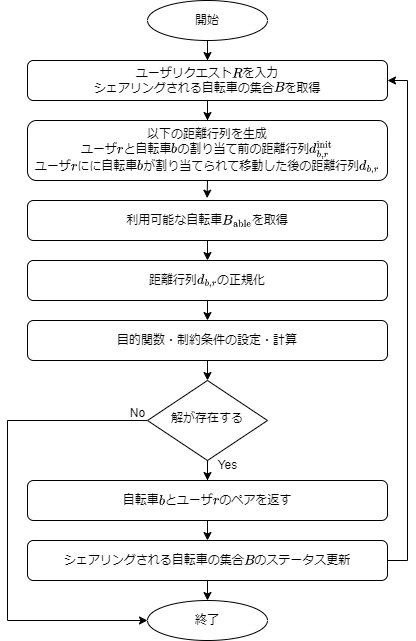
\includegraphics[scale=0.55]
            {figures/algorithmImplementation.png}
            \caption{自転車割り当てアルゴリズムのフローチャート}
            \label{fig:自転車割り当てアルゴリズムのフローチャート}
          \end{figure}

      \subsubsection{テストケースと結果(0\%)}
        \label{sec:テストケースと結果}
          \par  
  
  \subsection{機械学習モデルの実装(0\%)}
    \label{sec:機械学習モデルの実装}
      \par 
      
      \subsubsection{データセットの準備(0\%)}
        \label{sec:データセットの準備}
          \par
          
      \subsubsection{特徴量の選択と前処理(0\%)}
        \label{sec:特徴量の選択と前処理}
          \par
          
      \subsubsection{モデルの学習と評価(0\%)}
        \label{sec:モデルの学習と評価}
          \par
          
  \subsection{API開発(0\%)}
    \label{sec:API開発}
      \par
      
      \subsubsection{APIエンドポイントの実装(0\%)}
        \label{sec:APIエンドポイントの実装}
          \par
          
      \subsubsection{ドキュメンテーションとテスト(0\%)}
        \label{sec:ドキュメンテーションとテスト}
          \par
  % 第5章
    \clearpage
    \newpage
    % 第6章
\section{評価と結果(\textcolor{orange}{28\%})}
  \label{sec:評価と結果}
    \par
  
  \subsection{マッチングモデルの評価(0\%)}
    \label{sec:マッチングモデルの評価}
      \par
  
      \subsubsection{数理最適化モデルの結果分析(\textcolor{green}{100\%})}
        \label{sec:数理最適化モデルの結果分析}
          \par 本項では,\ref{sec:数理最適化モデルの実装}節にて定式化及び実装を行った数理最適化ベースの割り当てモデルを用いて,実際のデータを用いたシミュレーションを行い,検証する.
          \par シミュレーションでは,タクシー・リムジン委員会(LTC)より提供されているニューヨーク市のタクシーのトリップデータ\scalebox{0.7}{\cite{YellowTaxiTripRecords}}を用いる.CtoCシェアサイクルサービスは今日までサービスとして提供されていないため,実運用されているデータを用いた検証を行うことは難しい.そのため,任意の2地点間を自由に移動できるという点で,ユーザの需要傾向に相関があると考え,タクシーの実運用データを利用することとした.シミュレーションを行う期間は2023年1月1日の0時から24時までの24時間である.この期間内に合計約7.7万のリクエスト数が存在している.自転車に関しては,ニューヨーク市内にランダムに10台配置した.検証上,簡単のため自転車台数は10台と少なくしている.
          \par シミュレーションを行う手順として,簡単な例を図とともに説明する.
          \par まず,図\ref{fig:割り当て前のユーザと自転車の初期状態}に示すように,ある任意の1分間に3人のユーザからの利用リクエストがストックされたとする.その際のユーザの位置を橙色のアイコンでプロットしている.また,その際の利用可能な自転車の配置状況も緑色のアイコンでプロットしている.これが割り当て処理を行う前のユーザと自転車の初期状態である.
          \par 次に,図\ref{fig:半径250mの自転車を対象とする制約}に示すように,制約条件を満たしているかどうかの確認を行う.ユーザから半径250m圏内に駐輪されている自転車のみを割り当ての対象としているため,その圏外に駐輪されている自転車はグレーアウトし,割り当ての対象として処理されない旨を表している.
          \par 図\ref{fig:ユーザの進行方向と自転者オーナの方向}では,割り当て処理のためのパラメータとなるユーザの進行方向と,自転車とその自転車オーナの方向を取得している.ユーザの場合,それぞれのユーザの現在地から目的地までを実線で表現している.自転車の場合,それぞれの自転車からその自転車のオーナの家までを破線で表現している.破線が表現されていない自転車は既にオーナの元に駐輪されていることを意味している.
          \par 最後に,割り当て処理を実施し,図\ref{fig:割り当て処理結果}に示すような割り当て結果となる.この図では,自転車とユーザの色は割り当て成功後のペアに対応している.数理最適化処理を行ったことによって,図中央にいるユーザには,半径250m圏内に自転車が駐輪されているものの,目的地方向がその自転車のオーナ方向との真逆であったことから割り当てられなかったことが分かる.
          \par そして,これと同様の処理を24時間分のトリップデータに対して行う.24時間の時間経過による自転車全体のステータスの変化を表した結果が図\ref{fig:自転車の割り当て成功率とステータスの変化}である.青色のグラフは,それぞれの1分間のリクエストストックに対して,どれくらいの割合で自転車が割り当てられたかを示している.緑色のグラフは,全体の自転車に対してどれくらいの自転車が現在利用中であるかを示している.赤色のグラフは,全ての自転車をオーナの元に戻す際の再配置コストを示しており,実態は,各自転車とオーナとの距離の総和で,自転車の散らばり具合を表す.

          \begin{figure}[htbp]
            \centering
            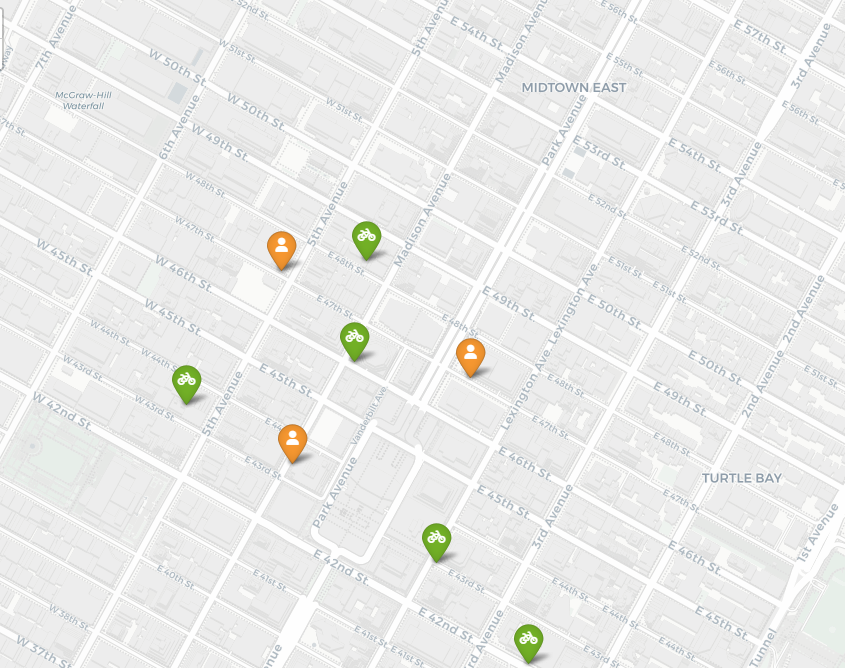
\includegraphics[scale=0.35]
            {figures/simulation1.png}
            \caption{割り当て前のユーザと自転車の初期状態}
            \label{fig:割り当て前のユーザと自転車の初期状態}
          \end{figure}

          \begin{figure}[htbp]
            \centering
            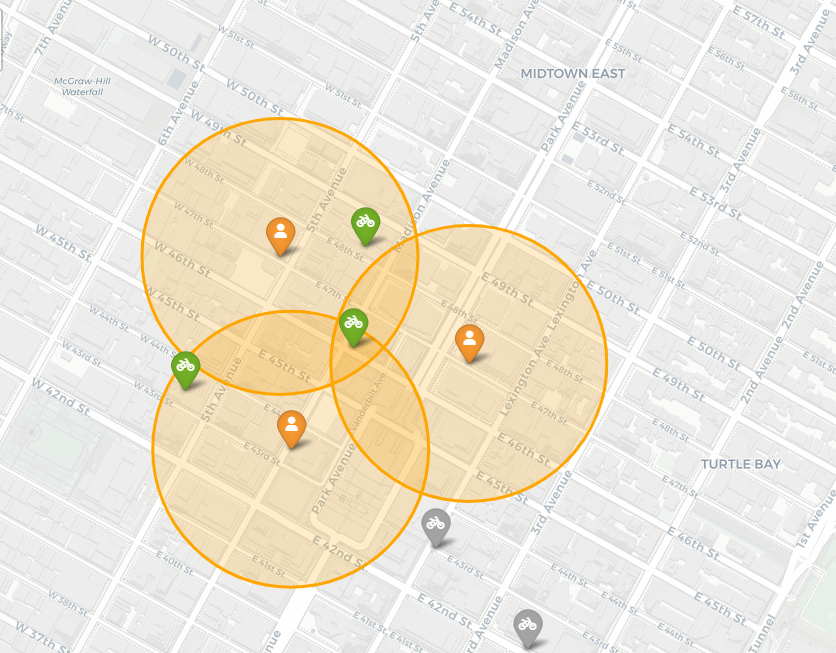
\includegraphics[scale=0.35]
            {figures/simulation2.png}
            \caption{半径250mの自転車を対象とする制約}
            \label{fig:半径250mの自転車を対象とする制約}
          \end{figure}

          \begin{figure}[htbp]
            \centering
            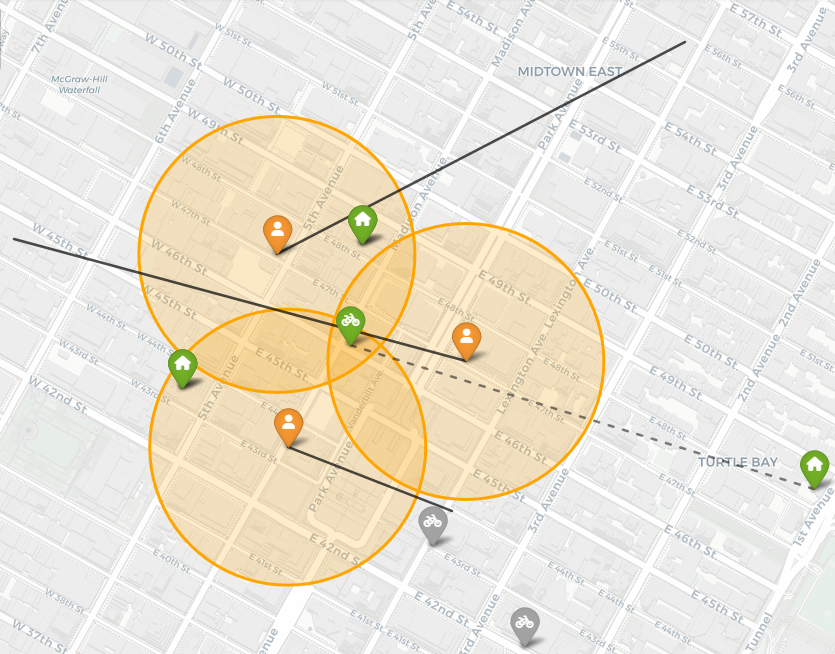
\includegraphics[scale=0.35]
            {figures/simulation3.png}
            \caption{ユーザの進行方向と自転者オーナの方向}
            \label{fig:ユーザの進行方向と自転者オーナの方向}
          \end{figure}

          \begin{figure}[htbp]
            \centering
            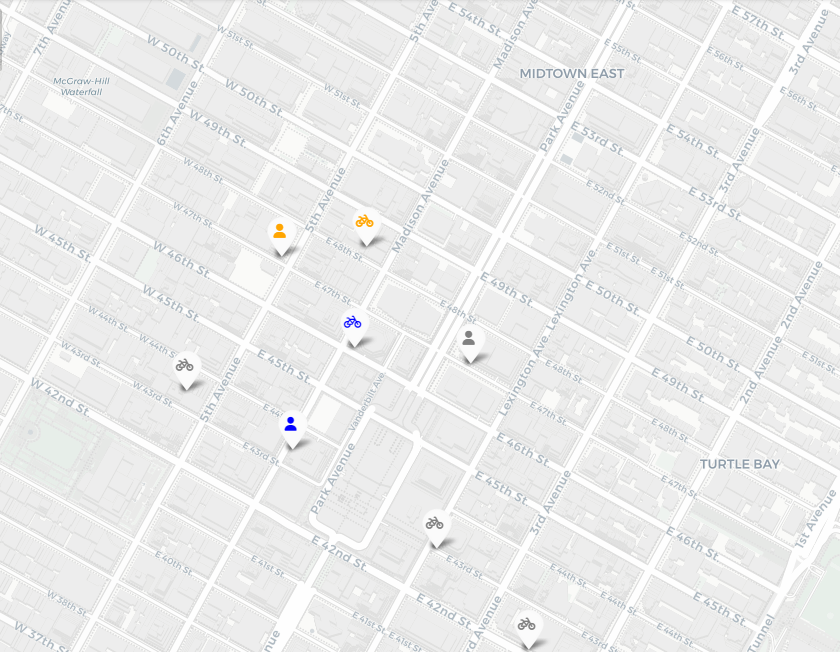
\includegraphics[scale=0.35]
            {figures/simulation4.png}
            \caption{割り当て処理結果}
            \label{fig:割り当て処理結果}
          \end{figure}

          \begin{figure}[htbp]
            \centering
            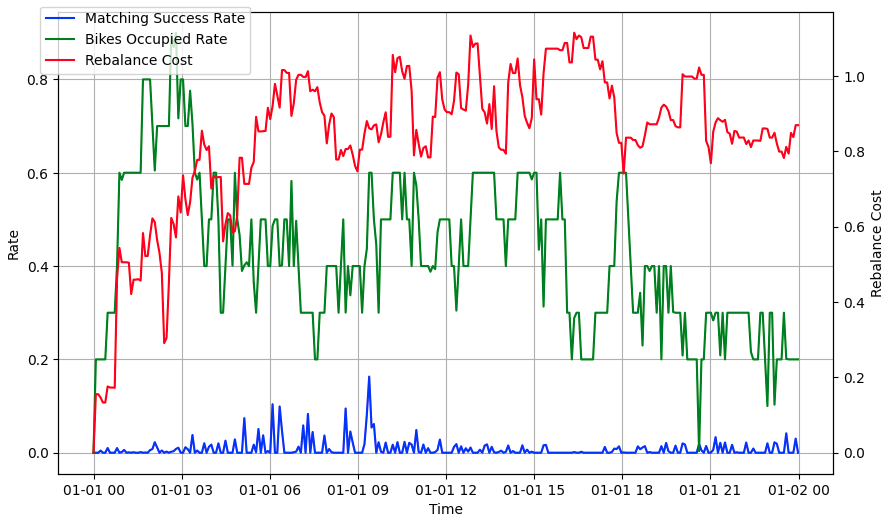
\includegraphics[scale=0.25]
            {figures/dispatchedResultFor1Day.png}
            \caption{自転車の割り当て成功率とステータスの変化}
            \label{fig:自転車の割り当て成功率とステータスの変化}
          \end{figure}

      \subsubsection{テストケースと結果(\textcolor{green}{100\%})}
        \label{sec:テストケースと結果}
          \par これまで,\ref{sec:数理最適化モデルの実装}節にてモデルの定式化やソルバーへの実装手順を示し,\ref{sec:数理最適化モデルの結果分析}項にて実際のデータを用いたシミュレーションを行った.本項では,それら実装したモデルやシミュレーションの妥当性の確認や解の品質評価を目的として,入力に対する出力の結果が意図する結果となっているかどうかを,テストケース及びテストコードを用意し,機械的に検証する.
          \par 数理最適化モデルが妥当な性能を発揮するかどうかを確かめるため,大きく分けて3種類のテストケースを用意する.それぞれ,小規模・中規模・大規模なデータである.小規模データでは,2台の利用可能な自転車が配置されている状態に対してユーザリクエストが1つ存在する状況のテストケースである.中規模データでは,5台の利用可能な自転車が配置されている状態に対してユーザリクエストが3つ存在する状況のテストケースである.大規模データでは,20台の利用可能な自転車が配置されている状態に対してユーザリクエストが10存在する状況のテストケースである.
          \par テストケースとして作成する自転車とユーザリクエストは,テスト観点を満たすための最低限のパラメータを持たせる.自転車は,現在地・自転車オーナの位置・利用終了予定時刻をパラメータとして持つ.ユーザリクエストは,利用開始位置・利用終了位置・利用開始時間・利用終了時間をパラメータとして持つ.また,\ref{sec:数理最適化モデルの結果分析}項のシミュレーションとは分離したテストを行うことでより妥当性が保証されるため,ニューヨークではなく東京周辺に自転車を配置したテストデータとする.
          \par 小規模データに関しては,さらに細かくテストケースを分割する.割り当てが成功する正常系と割り当てが失敗する異常系,制約条件を明らかに満たしていない例外ケースの3パターンを用意する.割り当てが失敗する異常系のテストケースは,表\ref{tab:小規模テストデータA及びBの自転車}及び表\ref{tab:小規模テストデータAのユーザリクエスト}に示す通りであり,これをテストデータAとしている.東京駅と新宿駅に2台の利用可能な自転車が駐輪されている状態で,東京駅から新宿駅までのユーザリクエストが存在しているシチュエーションである.結果としてユーザに自転車が割り当てられなかった.
          \par 割り当てが成功する正常系のテストケースは,表\ref{tab:小規模テストデータA及びBの自転車}及び表\ref{tab:小規模テストデータBのユーザリクエスト}に示す通りであり,これをテストデータBとしている.自転車の状態に関してはテストデータAに同じであるが,ユーザは,新宿駅から渋谷駅に向かいたいとする場合である.結果として新宿駅に駐輪されている自転車が割り当てられた.
          \par ここで,テストデータA及びBに関して,目的関数のパラメータを操作することによって,いかようにもなることが想定される.そのため,テストコード上で厳密に解の一致を判定することは行わず,想定しないエラーが発生せずに処理が完了することをテストしている.また,テストケースをカスタマイズして実際の挙動を確認する意義も果たしている.ただし,制約条件を明らかに満たしていない例外ケースはその限りではない.その場合はユーザに自転車が割り当てられるべきではないため,その旨が完全一致することをテストコード上で表現する.
          \par 具体的には,自転車の配置を表\ref{tab:小規模例外テストデータの自転車}に,ユーザリクエストは表\ref{tab:小規模テストデータAのユーザリクエスト}に示した通りのシチュエーションである.ユーザの利用開始位置に対して,自転車が明らかに制約条件を満たさない遠い距離に駐輪されている状態や,利用終了予定時間が未来である状態をテストしている.
          \par 小規模テストデータAやBと同じ要領で中規模データや大規模データに関してもテストケースを作成し,テストコードで機械的にテストを行えるよう整備した.データが大きくなるため,小規模データの説明の際に示したような表は割愛するが,付録のソースコードで確認できるため参照されたい.全てのテストケースに対して,それぞれ成功した場合は「SUCCESS」,失敗した場合は「FAILURE」をターミナルに出力できるようテストコードを整えて実行した結果が図\ref{fig:割り当てモデルのテスト}に示す通りである.全てのテストにパスしている.

          \begin{table*}[t]
            \caption{小規模テストデータA及びBの自転車}
            \label{tab:小規模テストデータA及びBの自転車}
            \centering
            \begin{tabular}{|l|l|l|l|} \hline
              自転車の現在地 & 自転車オーナの位置 & 利用終了予定時刻 & 場所(参考) \\ \hline
              (35.6804, 139.7690) & (35.6804, 139.7690) & NaT & 東京駅 \\
              (35.6895, 139.6917) & (35.6895, 139.6917) & NaT & 新宿駅 \\ \hline
            \end{tabular}
          \end{table*}
          
          \begin{table*}[t]
            \caption{小規模テストデータAのユーザリクエスト}
            \label{tab:小規模テストデータAのユーザリクエスト}
            \centering
            \begin{tabular}{|l|l|l|l|l|} \hline
              利用開始位置 & 利用終了位置 & 利用開始時間 & 利用終了時間 & 開始場所->終了場所(参考) \\ \hline
              (35.6804, 139.7692) & (35.6895, 139.6917) & now() & now()+15mins & 東京駅->新宿駅 \\ \hline
            \end{tabular}
          \end{table*}

          \begin{table*}[t]
            \caption{小規模テストデータBのユーザリクエスト}
            \label{tab:小規模テストデータBのユーザリクエスト}
            \centering
            \begin{tabular}{|l|l|l|l|l|} \hline
              利用開始位置 & 利用終了位置 & 利用開始時間 & 利用終了時間 & 開始場所->終了場所(参考) \\ \hline
              (35.6895, 139.6917) & (35.6618, 139.7012) & now() & now()+15mins & 新宿駅->渋谷駅 \\ \hline
            \end{tabular}
          \end{table*}

          \begin{table*}[t]
            \caption{小規模例外テストデータの自転車}
            \label{tab:小規模例外テストデータの自転車}
            \centering
            \begin{tabular}{|l|l|l|l|} \hline
              自転車の現在地 & 自転車オーナの位置 & 利用終了予定時刻 & 場所(参考) \\ \hline
              (35.8, 139.8) & (35.8, 139.8) & now()+1day & 足立区内某所 \\
              (35.81, 139.81) & (35.81, 139.81) & now()+1day & 埼玉県草加市某所 \\ \hline
            \end{tabular}
          \end{table*}

          \begin{figure}[htbp]
            \centering
            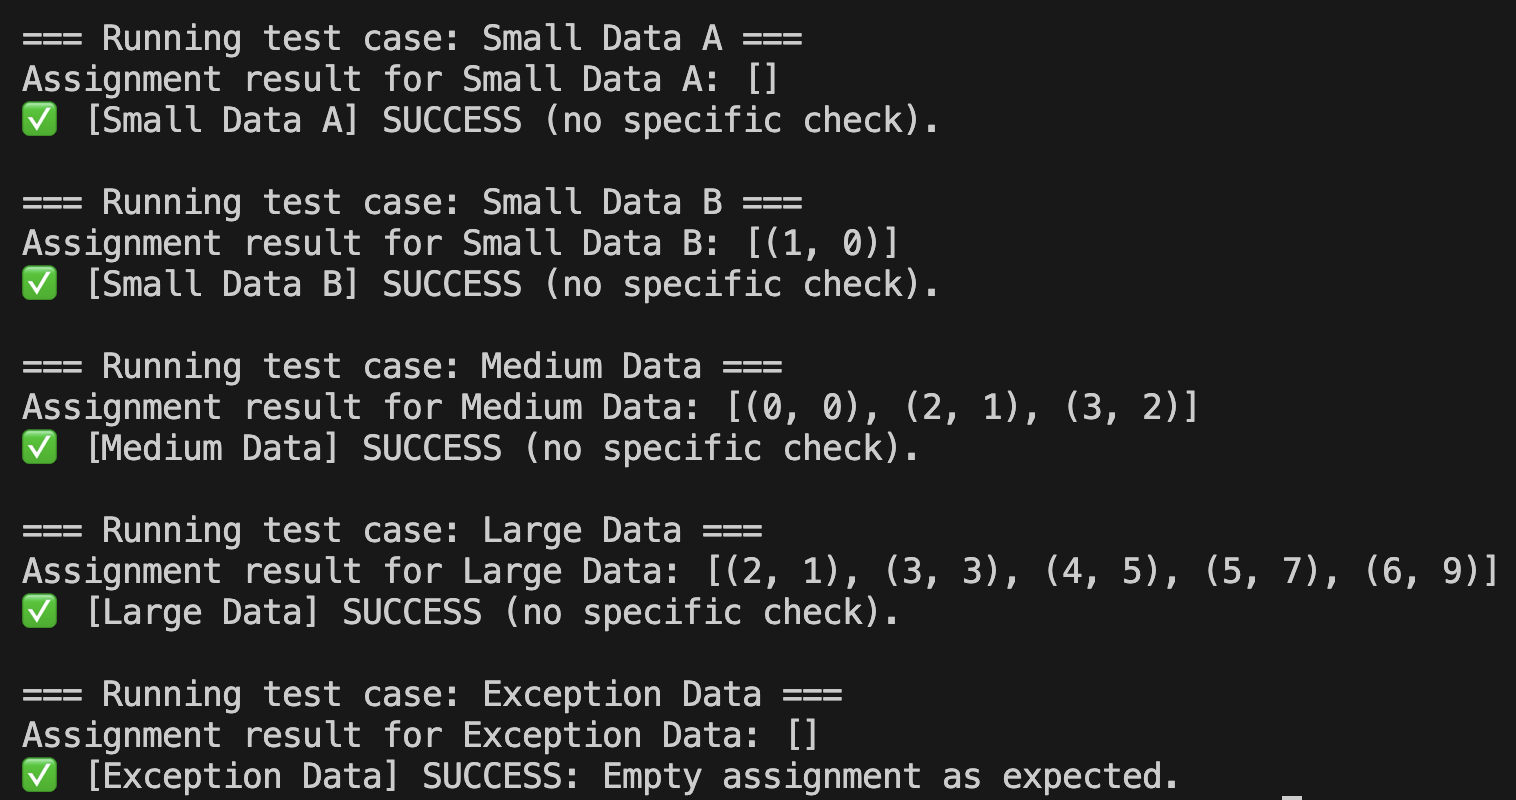
\includegraphics[scale=0.29]
            {figures/TestResult.png}
            \caption{割り当てモデルのテスト}
            \label{fig:割り当てモデルのテスト}
          \end{figure}

          
      \subsubsection{複数モデルの比較検討(0\%)}
        \label{sec:複数モデルの比較検討}
          \par
      
  \subsection{APIの適用性評価(0\%)}
    \label{sec:APIの適用性評価}
      \par
      
      \subsubsection{都市への展開シミュレーション(0\%)}
        \label{sec:都市への展開シミュレーション}
          \par $\Box$ 統合テスト
          \par $\Box$ エンドツーエンド(E2E)テスト
          
      \subsubsection{スケーラビリティとパフォーマンス評価(0\%)}
        \label{sec:スケーラビリティとパフォーマンス評価}
          \par $\Box$ 負荷テスト
  % 第6章
    \clearpage
    \newpage
    % 第7章
\clearpage
\newpage

\section{考察}
  \label{sec:考察}
    \par 本研究では,個人所有の自転車を対象としたCtoC型のドックレスシェアサイクルシステムを提案し,その有効性について検証を行った.以下では,システム全体の有効性,CtoC化によるメリットとデメリット,技術的課題と解決策,そして社会的インパクトと倫理的考慮について総合的に考察する.
    \par また,本研究は限定的な実験環境下で評価を行ったに過ぎないため,現場での利用状況や利用者からのフィードバックを踏まえたさらなる検証と改善が今後の大きな課題となることが示唆される.
    \par まず,システム全体の有効性については,\ref{sec:システム全体の有効性}節で詳述したとおり,実データを用いたシミュレーションにより再配置コストを評価指標として検証を行った.その結果,提案した数理最適化ベースの割り当てモデルが,自転車数をスケールアップした場合に特に有意な効果を示すことが明らかとなった.また,サービス提供開始から一定時間経過後においても,再配置コストが低い水準で推移することがかくにんできた.これらの結果は,提案システムが長時間運用や大規模展開に適している可能性を示唆している.
    \par 次に,CtoC化によるメリットとデメリットについては,\ref{sec:CtoC化によるメリットとデメリット}節で述べたとおり,サービス利用者と自転車提供者の双方に利点が存在する.利用者側では,ドックレスかつ乗り捨て可能なシステムにより,移動の自由度が向上し,都市部だけでなく地方でもサービス利用が可能となる潜在性がある.一方,提供者側では,自転車のアイドルタイムを有効活用することで収益を得られる利点がある.しかしながら,待ち時間の発生や盗難リスクといった問題点も指摘でき,これらへの対策が必要不可欠である.
    \par 技術的課題と解決策については,\ref{sec:技術的課題と解決策}節で検討したように,数理最適化モデルとスマートロックの連携が最優先の課題として挙げられる.また,支払処理機能や評価・レビュー機能の実装もサービスの信頼性向上のために重要である.さらに,大規模なシミュレーションを行う際の計算リソースの制約も明らかとなったため,GPU環境の活用などによる効率的な計算資源の確保が求められる.
    \par 社会的インパクトと倫理的考慮に関しては,\ref{sec:社会的インパクトと倫理的考慮}節で述べたとおり,不法駐輪問題や自転車の放置などの社会的課題が懸念される.また,自転車提供者のプライバシー保護や盗難防止策の徹底など,倫理的観点からの配慮も重要である.これらの課題に対しては,規制当局やコミュニティとの共同による適切なルール作りや,技術的なソリューションの導入が求められる.
    \par 加えて,本システムは新たなモビリティサービスとして利用者の利便性向上に寄与するだけでなく,地域経済の活性化や環境負荷の低減といった広範な社会的効果も期待できる.
    \par 総合的に,本研究の提案システムは,新しいモビリティサービスの形態として有望である一方,多方面にわたる課題解決が必要であることが示唆された.今後は,技術的課題の克服とともに,社会的・倫理的側面における対策を講じることで,持続可能なサービスの実現を目指す必要がある.また,数理最適化モデルのさらなる改良や大規模データでの検証を進めることで,システムの実用性を高めていくことが期待される.
  
  \subsection{システム全体の有効性}
    \label{sec:システム全体の有効性}
      \par まずはじめに,本研究全体を通して取り組んだ課題やその目的について改めて簡単にまとめる.本研究では,比較的偏りが少なく,各地に点在している個人所有の自転車に焦点を置き,そのリソースを有効活用して社会全体としてのモビリティ体験を向上させることを目的として,個人間で自転車をシェアリング可能とするCtoCでドックレスなシェアサイクルシステムを提案し,実装した.
      \par そのため,システムを実装後の実データを用いたシミュレーションの際には,自転車の散らばり具合を再配置コストと命名し,それを最重要評価指標として設定し,評価を行った.その結果の1つが図\ref{fig:モデル別再配置コストの時間経過比較}である.
      \par しかし,前述している通り,検証時の状態は,ニューヨーク市内に自転車を10台ランダム配置した状態であり,明らかにユーザリクエストによる需要に対して自転車の供給が足りていない状況であり,再配置コストの推移が現実的なものであるかどうか判断しかねる結果となっていた.実際に,図\ref{fig:自転車の割り当て成功率とステータスの変化}から分かる通り,割り当て成功率が高くない.ニューヨーク市内の7万以上のタクシーデータに対して10台の自転車しか用意していないからである.
      \par そこで,初期配置する自転車を50台にスケールアップして同様にシミュレーションを行ってみた結果が図\ref{fig:50台の時の再配置コストの時間経過比較}であった.ただし,初期配置する自転車を50台にスケールアップした場合でも,やはり7万以上のユーザリクエストに対しては非常に不足している状態であるため,割り当て成功率の上昇には期待できなかった.それでも,スケールアップ前と後で再配置コストの推移の結果を見比べてみると,その違いが顕著に表れるようになった.24時間継続してサービスを提供した後の再配置コストは,バッチ最適化割り当てモデルを除いた全てのモデルが同じような値に収束していることが分かる.一定期間経過後は,バッチ最適化割り当てモデルが他のモデルと比較し,低い水準で再配置コストが推移している.
      \par さらに,初期配置する自転車を100台にスケールアップして同様にシミュレーションを行ってみた結果が図\ref{fig:100台の時の再配置コストの時間経過比較}であった.この場合でも変わらずバッチ最適化割り当てモデルが他のモデルと比較し,低い水準で再配置コストが推移していることが読み取れるが,自転車の初期配置数を10台から50台へとスケールアップした場合と比べて,50台から100台へのスケールアップは,別の割り当てモデルとの差が倍率としてそれほど開くことはなかった.
      \par これらの結果から,24時間継続してサービスを提供した場合,本研究で提案した数理最適化ベースの割り当てモデルが有意であることが分かる.また,基本的には,自転車数をスケールアップした場合の方が,再配置コストにより有意性が増しているため,スケールメリットを持つ割り当てモデルであることが期待される.しかし,より細かなスケール幅で自転車数を増減させて検証し,詳細な結果をまとめる必要があるが,ある一定数の自転車数を超えるとそれ以上のスケールメリットは享受できない可能性も示唆される.
      \par さらに,自転車を10台初期配置した場合の結果である図\ref{fig:モデル別再配置コストの時間経過比較}から,サービス提供開始後8時間までは,逐次最適化割り当てモデルとバッチ最適化割り当てモデルとで再配置コストに大きな違いは見られなかった.逐次最適化割り当てモデルは文字通り,1リクエストずつ処理し,自転車の割り当てを行うため,ユーザに待ち時間を発生させないというメリットがある.そのため,CtoC事業者側が状況によってより最適なモデルを選択できるという考察もできた.しかし,50台にスケールアップした状況下においていは,逐次最適化割り当てモデルはサービス提供開始直後から再配置コストが比較的急激な上昇を見せているため,その限りではないことが読み取れる.より大規模な自転車データを準備した状態で検証し,それらの仮説を明らかにしていく必要がある.
      \par 数理最適化モデルの定式化の観点からも考察したい.数理最適化ベースのマッチングモデルを設計する際に,その目的関数を\ref{equ:目的関数}式と定義した.この式は,「ユーザが,割り当てられた自転車に乗って移動した後の自転車とその自転車の所有者までの距離を最小化」することと,「可能な限り多くのユーザに自転車を割り当てる最大化」することに対するトレードオフを重みを掛け合わせることで調整している.本研究では,簡単のため,この重みを1に固定して実装しているが,この重みの最適解を探る検証も不可欠である.
      \par また,シミュレーション検証において,本研究ではモデルの検証のため,ニューヨーク市のタクシーデータを用いたが,自転車に比べてタクシーは移動距離が大きくなると考えられる.つまり,実際のCtoCシェアサイクルサービスを想定した場合,タクシーよりも移動距離が短く,範囲も限定されることから,シミュレーションを行なった結果よりもより小さい値でリバランスコストが推移する可能性も十分考えられる.
      \par さらに,今後実証実験の環境を整えることができれば,実際の運用環境から得られるリアルタイムデータを活用することで,より柔軟なパラメータ調整やアルゴリズムの改良が期待できると考えられる.
      
  \subsection{CtoC化によるメリットとデメリット}
    \label{sec:CtoC化によるメリットとデメリット}
      \par 本研究にて提案したシステムによってCtoC化を実現することによるメリットは,サービス利用者と自転車提供者の双方にある.サービス利用者側においては,乗り捨て可能なシステムを前提としていることから移動自由度が大きく上昇することが期待される.また,従来のシェアサイクルサービスが豊富に展開されいている都市部に限らず,地方でもサービスを利用することができる可能性を秘めている.
      \par 自転車提供側においては,自身の自転車を利用していない時間帯にその自転車を有効利用できる点にある.アイドルタイムが発生する対象に対してシェアリングすることで,提供者側は,いわゆる不労所得を得ることができる.また,シェアリングした自転車が乗り捨てされる場合,一時的に所有者のもとに返却されないものの,数理最適化アルゴリズムによる割り当て処理を行っていることから,所有者の元に自動的に返却される,もしくはその近くに駐輪される可能性が高いため,所有者が利用したい場合もスムーズに対応できることが期待される.
      \par 一方で,本研究にて提案したシステムによってCtoC化を実現することによるデメリットも存在する.サービス利用者側においては,待ち時間の発生にある.図\ref{fig:モデル別再配置コストの時間経過比較}や図\ref{fig:50台の時の再配置コストの時間経過比較}を参照してみると分かる通り,逐次最適化割り当てモデルよりもバッチ最適化割り当てモデルの方が再配置コストが低い.本研究の場合,バッチ幅は1分間としており,1分間のユーザリクエストをストックすることとなる.ある1分間に対して,毎秒のリクエストが送られてくる確率が同様に確からしいとすると,ユーザはリクエストを行ってからレスポンスが返ってくるまでに平均して30秒間待機する必要があることになる.
      \par 実験的にストックする時間を1分として実装しているが,ユーザの平均待機時間が30秒であることは,ユーザ体験として良いとは言えない.さらに,ユーザリクエスト数や提供される対象の自転車数が大規模であった場合,数理最適化割り当て処理自体にも処理時間が発生し,30秒以上待機する必要がある.一方で,システム全体としては,リクエストをストックする時間に応じて数理最適化の旨味が増し,再配置コストが低い結果を得ることが期待される.このように,ユーザ体験とシステム効率のトレードオフを探るにあたって,リクエストをストックする時間幅の最適解も探る必要がある.
      \par 自転車提供側においては,自身の自転車が盗難される危険性がある点がデメリットになり得るだろう.自転車の鍵はスマートロックで管理し,対象のユーザはそのスマートロックを解錠できることになる.悪意のあるユーザに利用されてしまった場合,簡単に自転車を盗難できる状況が発生する.利用する前のユーザ登録時などに厳正な個人認証を行い,盗難を働きかけたとしてもすぐに特定できる仕組みや抑止力が必要であると考えらえる.
      \par さらに,本システムの普及は,利用者の移動の利便性向上に加えて地域経済の活性化や環境負荷の低減といった社会的メリットをもたらす可能性がある一方,地域ごとの交通ルールや文化に即した運用方法の検討が不可欠となる.
      
  \subsection{技術的課題と解決策}
    \label{sec:技術的課題と解決策}
      \par 技術的課題として最もコアな点は,自転車割り当てモデルとスマートロックが未結合である点が挙げられる.APIを実装したものの,構築した割り当てモデルを利用するためのインターフェースにしかすぎず,割り当て処理を行った結果からスマートロックと連携し,解錠及び施錠の操作を行うまでの実装には至らなかった.一連のシステムとして大成するためにはこの連携は急務の課題である.
      \par また,他にも,設計したものの実装まで至ることはできなかった機能として,支払処理機能や評価・レビュー機能が挙げられる.これらも,スマートロック連携よりはプライオリティが下がるものの,必要不可欠な機能の1つであるためAPIのマイクロサービスの1つとして実装してく必要がある.
      \par 構築した自転車割り当てモデルを用いてシミュレーション実験を行う際にも技術的課題に直面した.計算リソースの不足である.大規模なケースとして,ニューヨーク市内に650台の自転車を初期配置したシチュエーションでのシミュレーションを試みたが,かなりの時間的計算コストを要し,結果を取得するまでに至らなかった.CPU環境を用いた実験環境を構築したことが,時間的計算コストを要した一因として考えられるため,GPU環境を用いた実験環境の構築と,GPUリソースを最大限生かすことのできるシミュレーションのソースコード修正が必要になると考えられる.
      \par さらに,システム全体のセキュリティ対策の強化や不正利用防止のための監視機能の充実も,今後の実装において重要な検討項目として挙げられる.
      
  \subsection{社会的インパクトと倫理的考慮}
    \label{sec:社会的インパクトと倫理的考慮}
      \par 本研究にて提案したシステムをサービスとして社会実装するとなった際に考え得る社会的影響として,自転車の放置問題が挙げられる.ドックレスでどこでも乗り捨て可能なシステムとしているからである.実際に既存のドックレスシェアサイクルサービスでも駐輪場の不足や,それによって自転車が歩行者用通路にはみ出して駐輪されている問題も散見される.本研究のサービス設計では,そうした課題がより顕著に表れる可能性も十分に想定される.
      \par また,実現可能性についてもまだまだ課題がある.本研究で提案した数理最適化ベースの割り当てモデルの設計を行う際に,前提条件として,自転車はどこでも乗り捨てが可能であることとし,乗り捨てによる法的な側面の課題はモデル構築において考慮しないと言及している.しかし,実社会でサービス提供を行う際には最もネックになる部分であると考えられる.
      \par さらに,サービスを利用するユーザのプライバシー保護にも重点を置かなければならない.特に,自転車提供側はその自転車のあるべき駐輪場の位置情報を共有するべきであるが,それがそのユーザの住所である可能性も大いに考えられ,どのように自転車利用者にそれを公開するのか,安全な方法を検討しなければならない.
      \par \ref{sec:CtoC化によるメリットとデメリット}節でも述べた盗難に関する課題やここで述べた不法駐輪等の公共道路に関する課題・ユーザのプライバシー保護などの倫理的に考慮しなければならない点は,より詳細を詰めて考える必要がある.
      \par さらに,利用者間の信頼性向上や情報公開の透明性を確保する仕組みの導入,及び地域ごとの法制度や規制に柔軟に対応するためのガイドライン整備も,今後のサービス実現に向けた重要な課題として認識される.
  % 第7章
    \clearpage
    \newpage
    % 第8章
\section{結論と今後の展望(\textcolor{green}{100\%})}
  \label{sec:結論と今後の展望}  
    \par 本研究では,CtoCドックレスシェアサイクルの実現を目指し,その可能性についての議論や,具体的なビジネスモデルの検討,技術的要件の抽出やシステムの実装を行なった.全章を俯瞰すると,まず関連研究の整理を行った.ここではシェアサイクルの現状や課題,研究で必要となるスマートロックやマッチングアルゴリズムなどの技術的な研究動向についても多くの文献を参考にし,本研究の立ち位置を明らかにすることにも繋がった.その後,CtoCシェアサイクルのサービス設計とビジネスモデルを定義し,本研究の対処となるドメイン領域への理解を深めたり,既存サービスとの差別化を行ったりした.
    \par 続く章にて,システムの設計や実装を行なった.設計では要件定義に始まり,サービスとして価値提供するにあたって将来的に必要となる機能も考慮しながら必要事項をまとめた.設計内容を実装するにあたっては,本論文を読んでシステム構築を再現することができるよう可能な限り具体的に手順を紹介した.構築したモデルに対しては,実際のニューヨーク市のタクシートリップデータを利用しシミュレーション実験を行なった.サービス提供後の自転車の再配置コストを最重要評価指標に設定し評価を行なった結果,本研究で構築した自転車割り当てモデルが最も有意な結果を得ることができた.またその結果に対する考察も続く章にて行なった.
    \par 本研究全体を通して振り返ると,CtoCドックレスシェアサイクルの実現には至らなかったものの,そのコア要素となる自転車の割り当てモデルは十分な性能を発揮するモデルを構築できたと言える.また,既存のBtoC型シェアサイクルサービスやそれらに関わる研究が中心の中で,CtoC型に特化したサービス提案や数理最適化をベースとした自転車割り当てモデルの構築,それに伴う自転車のスマートロックのプロトタイプ提案を行なった点も本研究の貢献である.
    \par それでも,今後の考慮していかなければならない課題は山積みである.例えば,地理的制約を追加する必要がある点である.本研究で構築した自転車の割り当てモデルのアルゴリズムでは,障害物の無い平面上として処理を行なっている.しかし,現実世界では多様な障害物が存在する.あるユーザからのリクエストに対して直線距離的にすぐ近くに適切な自転車が駐輪されていたとしても,ユーザと自転車の間は河川で隔てられており,自転車の場所までユーザが到達するためには,回り道をして橋を渡らなければならないなどの状況がその一例である.この場合,ユーザ体験が非常に悪化することになりかねない.対処方法の一案としては,サードパーティ製のAPIを利用し,二地点間の道のりによる距離を取得した上で割り当て処理を行う方法が考えられる.現実世界における地理的制約は複雑であるもののクリティカルな課題であるため,CtoCドックレスシェアサイクルの実現のためには避けて通ることはできないだろう.
    \par また,時間制約を追加しなければならない点もまだ残されている課題である.本研究にて行なったシミュレーションでは,初期配置している自転車の全てが,24時間オーナが利用せず,他のユーザが利用していない限りシェアリングの対象となることを前提として行われている.しかし実際には,自転車オーナは12時間後に自身で利用する予定があるかもしれないし,サービス提供開始後数時間経ってからシェアリングの対象として貸し出すことができるようになるかもしれない.シミュレーション自体はシンプルであることに意義があるため,過剰な考慮事項になるかもしれないが,シチュエーションとしては対処できなければならない項目であるため,これも,CtoCドックレスシェアサイクルの実現のためには避けて通ることはできない.
    \par 他にも,ユーザの選好を元にした優先度や特定の条件を反映する制約の追加も必要である.例えば,ユーザがクロスバイクを利用したいと考えているのか,もっとシンプルな自転車で事足りるかなどの条件で割り当てる自転車を考慮しなければならない点がその一例である.
    \par 今後の展望として,上記の課題に対するアプローチや法的側面における課題などをクリアし,実証実験等に取り組むことができればより面白い研究に発展していくことができると期待している.CtoCのシェアリングであることを最大限活かし,オーナが自由に,自転車の利用のための時間単価を設定したり,人気の自転車の場合には,ユーザ側が価格を押し上げて提案する方式や機能があっても面白いかもしれない.本研究をきっかけとして,CtoCドックレスシェアサイクルが実現できることを切に願っている.モビリティ体験のさらなる向上に思いを馳せて.
  % 第8章
    \clearpage
    \newpage

    \onecolumn
    % 参考文献
    \bibliographystyle{junsrt}
    \bibliography{references}
    \clearpage
    \newpage
    
    % 付録
    \appendix
    \section{付録}
  \label{付録}
    \subsection{ESP32 DEVKIT V1のピン番号レイアウト}
      \label{sec:ESP32 DEVKIT V1のピン番号レイアウト}
        \begin{figure}[htbp]
          \centering
          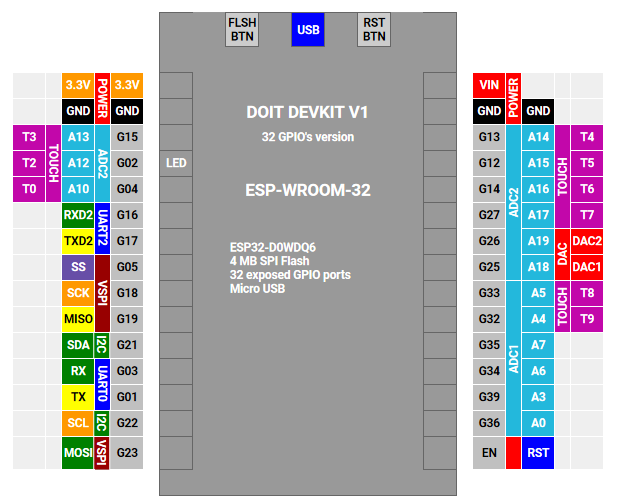
\includegraphics[scale=1]
          {figures/DOIT-DEVKIT-V1-32.png}
          \caption{ESP32 DEVKIT V1のピン番号レイアウト,Tim Sinaeve,beNative/ESP32-GPIO-list: ESP32 pinouts,DOIT modules in README.md.\cite{esppingithub}より引用}
          \label{fig:ピン番号レイアウト}
        \end{figure}
  
       \subsection{ソースコード}
        \label{sec:ソースコード}
         \par 別途,CD-ROMに実験に用いた全てのソースコードを添付する.具体的なディレクトリやコードの説明はルートディレクトリに保存するREADME.mdファイルを参照されたい.

       \subsection{API仕様書}
        \label{sec:API仕様書}
         \par 本研究で構築したAPI仕様書を添付する.ただし,ソースコードからローカルサーバを立ち上げ,ブラウザで表示させることでデバッグすることも可能であるため,そちらを推奨する.
    
       \subsection{情報処理学会予稿}
        \label{情報処理学会予稿}
         \par 別途,情報処理学会の発表内容の予稿を添付する.

       \subsection{紀要論文}
        \label{紀要論文}
         \par 別途,紀要論文を添付する.
    % \subsection{機械学習モデルの設計}
    %   \label{sec:machine_learning_model_design}
    %     \par

    % \subsection{機械学習モデルの実装}
    %   \label{sec:機械学習モデルの実装}
    %    \par 
      
    %   \subsubsection{データセットの準備}
    %     \label{sec:データセットの準備}
    %       \par
          
    %   \subsubsection{特徴量の選択と前処理}
    %     \label{sec:特徴量の選択と前処理}
    %       \par
          
    %   \subsubsection{モデルの学習と評価}
    %     \label{sec:モデルの学習と評価}
    %       \par
          
    % \subsection{機械学習モデルの結果分析}
    %   \label{sec:機械学習モデルの結果分析}
    %     \par


\end{document}

